\documentclass[conf]{new-aiaa}
%\documentclass[journal]{new-aiaa} for journal papers
\usepackage[utf8]{inputenc}
\usepackage[T1]{fontenc}
\usepackage{lmodern}
\usepackage{comment}
\usepackage{graphicx}
\usepackage{amsmath}
%\usepackage[numbers,super]{natbib}
\usepackage[version=4]{mhchem}
\usepackage{siunitx}
\usepackage{longtable,tabularx}
\setlength\LTleft{0pt} 
\usepackage{listings}
\usepackage[tableposition=top]{caption}
\usepackage{floatrow}
\floatsetup[table]{capposition=top}
\usepackage{xcolor}

\lstset{basicstyle=\small\ttfamily,columns=flexible,breaklines=true}

\title{A Case Study in Formal Specification and Runtime Verification of a CubeSat Communications System}
%\title{A Case Study in Formal Specification and Runtime Verification of a CubeSat Communications System}

\author{Zachary A. Luppen\footnote{Ph.D. Student, Aerospace Engineering, Iowa State University, Ames, Iowa, 50011, Student Member.} and Dae Young Lee\footnote{Assistant Professor, Aerospace Engineering, Iowa State University, Ames, Iowa, 50011, Member.} and Kristin Y. Rozier\footnote{Assistant Professor, Aerospace Engineering, Iowa State University, Ames, Iowa, 50011, Associate Fellow.}}
%\affil{Iowa State University, zaluppen@iastate.edu}
%\author{Dae Young Lee\footnote{Assistant Professor, Aerospace Engineering, Iowa State University, Member.}}
%\affil{Iowa State University, daylee@iastate.edu}
%\author{Kristin Y. Rozier\footnote{Assistant Professor, Aerospace Engineering, Iowa State University, Associate Fellow.}}
%\affil{Iowa State University, kyrozier@iastate.edu}

%\author{Zachary A. Luppen \footnote{Ph.D. student, Aerospace Engineering, Iowa State University, Ames, IA, 50010, USA.}}
%\affil{Iowa State University, Ames, Iowa, 50011, USA.}
%\affil{Iowa State University, Ames, Iowa, 50011, USA.}
%\author{Kristin Y. Rozier \footnote{Assistant Professor, Aerospace Engineering, Iowa State University, Ames, IA, 50010, USA.}}
%\author{Dae Young Lee \footnote{Assistant Professor, Aerospace Engineering, Iowa State University, Ames, IA, 50010, USA.}}
\affil{Iowa State University, \{zaluppen,kyrozier,daylee\}@iastate.edu}

\begin{document}

\maketitle

\begin{abstract}

CubeSats are garnering a lot of attention from several research communities due to their cheap price and easy accessibility to space. Although a CubeSat offers the potential to replace large and complex satellites for various space missions, developing a high-integrity platform that can fly in space requires robust software performance. The communications system of a CubeSat %and space systems 
%-- and any other spacecraft mission for that matter -- 
is critical to mission success. However, failed communications to the ground stations are commonplace for CubeSat projects. Thus robustifying against these potentially mission-ending failures poses one of the leading challenges for CubeSat missions both now and in the future. %The ability to detect faults in a CubeSat's communications system would aid in preventing a premature mission end as well as carry on the hard work performed by the developers.
Runtime verification (RV) specializes in real-time error detection in these types of temporal, reactive systems, and the R2U2 verification engine proved to fit in the CubeSat's resource constraints. We design specifications to detect and trigger appropriate mitigations for communications system faults. We discuss communications system specification debugging, validation, and variable coverage. Experimental evaluation on simulated orbital and telemetry datasets demonstrates that running R2U2 within a CubeSat communications system would detect several unique faults and trigger mitigations for these such as atypical position measurements or a voltage supply failure from occurring. We provide a roadmap from large CubeSat datasets to specification patterns for automatically capturing common monitoring properties. We outline our plans for integrating RV into other CubeSat systems as well as verifying an entire CubeSat telemetry dataset.

\end{abstract}

%%%%%%%%%%%%%%%%%%%%%
%% Nomenclature
%%%%%%%%%%%%%%%%%%%%%

%%%%%%%%%%%%%%%%%%%%%
\section{Introduction}
%%%%%%%%%%%%%%%%%%%%%

Over the past decade, the use of CubeSats and other nanosatellites by academic, governmental, commercial, and amateur entities has grown drastically \cite{cubesat101,Poghosyan2016,Villela2019}. The relatively low cost and fast development times of these projects make a CubeSat an ideal platform for experimenting in space \cite{cubesat101}. As of June 2020, over 1,300 CubeSats have been launched into space \cite{Kulu2020}. CubeSats may offer a scaled-down, simplified platform for developers, but they still experience many of the same and more problems that large satellites do \cite{Improving2017}. Design flaws, poor workmanship, software bugs, low reliability of hardware (often consisting of commercial off-the-shelf (COTS) components), lack of adequate testing, and communications failures are among a few of the many problems CubeSat projects experience \cite{Improving2017}. 
The low cost and short development times for these missions are appealing to space researchers;
 their use is only expected to rise in the coming years \cite{Improving2017,cubesat101}, so it is important that we find ways to mitigate their faults, within CubeSat resource constraints. 

The communications system of a CubeSat is vital to mission success. A CubeSat could be performing invaluable science, but a failure to communicate the results back to the ground renders the mission pointless. Communications system failures are currently one of the most common problems experienced by CubeSat developers \cite{Improving2017,Langer2016}. Enabling a CubeSat to monitor for these faults in real-time on-board would enable the CubeSat to either automatically trigger mitigation actions, or better utilize the satellite's limited bandwith to send specific fault information, rather than a large collection of unanalized data, to the ground. 
%Say that
%Enable the CubeSat to monitor for these faults in real-time on-board and use its limited bandwith to inform ground crew of a fault rather than sending large amounts of data to be better use of bandwith, better at trigger mitigatin.
Runtime verification (RV) specializes in identifying temporal fault signatures characteristic of communication systems faults. If we can specify a temporal fault signature using the data available on-board, then an RV engine can monitor for that fault. The CubeSat's strict power and computational constraints present a major impediment to embedding RV on-board. Any solution would need to operate with real-time guarantees, without dominating the system's resources, and provide the ability to reconfigure the monitors during system operation, without resynthesis, so that we can efficiently adapt to the dynamic operaitng environment after the CubeSat has launched. 
The Realizable, Responsive, Unobtrusive Unit (R2U2) tool is the only existing RV engine that satisfies all of our CubeSat system's constraints; it was specifically designed to provide flight-certifiable, resource-award RV that can be easily reconfigured post-deployment. 

% We can then
% CubeSats have strictly limited resources including low computing power so the RV engine needs to fit within those resources without consuming too much power and 

Recently, others have recognized the need to advance capabilities for CubeSat verification, which is now a pressing research topic. Analysis of these faults at design time via probabilstic model checking \cite{PLMJZ13}, and a model-driven trace-checking approach to elucidate on the most frequent requirement types in cyber-physical systems \cite{Boufaied2020} provide promising platforms for producing more robust CubeSat designs. Recently, \cite{Gross2020} formally verified a CubeSat's attitude, determination, and control system (ADCS) at design time and used this to cross-check the runtime behaviors of an unverified version. Now we must face the challenge of bridging the gap to on-board runtime verification, so that we can detect and mitigate any unexpected faults, e.g., due to the dynamic environment, that these previously-explored verification efforts could not anticipate at design time.

We examine a CubeSat communication system model and overview its design and implementation. The model consists of two separate systems, one consisting of orbital data (similar to information acquired by a ground station system) and the other comprised of telemetry information for a communications system module (simplified telemetry data with information such as voltages and temperatures). Using methods described in \cite{Roz16} and expanded upon in \cite{Cauwels2020}, we develop, revise and validate formal specifications for these two sub-systems and detail patterns observed during the process.
We encode these specifications as runtime observers using R2U2 and validate them against datasets generated by the model to ensure the absense of fault-positive fault alerts. To further validate their accuracy, we inject realistic faults -- such as unreasonable elevation and voltage measurements -- into the datasets at known times and check that R2U2 immediately detects these faults without false negatives, which NASA identifies as one of the most prominent issues in developing intelligent, autonomous systems \cite{Roadmap2015}. This case study provides a roadmap for developing a more robust CubeSat communications system through formal specification and details the process for integrating runtime verification (RV) into such a system to provide autonomous verification of its operation during operation.

Our contributions are as follows:

\begin{enumerate}
  \item We develop a reference set of formal specifications in mission-time linear temporal logic (MLTL) describing a modeled CubeSat communications system
  \item We detail our validation strategy over these specifications using experimental evaluation with the R2U2 tool
  \item We highlight and discuss specificaiton patterns that emerge while developing and revising the RV specifications
  \item We discuss lessons learned from validating these specifications that may inform future CubeSat runtime verificaiton efforts.
\end{enumerate}

This paper is organized as follows. Section II provides an overview of our communications system model, dividing. Section III contains our formal specifications, relating to information sourced from a CubeSat telemetry dataset as well as a ground station. For future developers, we elucidate on the organization of the specifications, the need for temporal operators, discuss coverage, and note specific patterns we encountered during their creation. Section IV describes our test scenarios and output graphs from R2U2 for a handful of our specifications. Section V concludes with lessons learned during the specification development and testing process and discusses future steps for RV integration into CubeSat systems and telemetry analysis.

% What do we do in this paper? So the contributions are, 1 Produce CubeSat communications system model.
% Develop a reference set of specifications in section 3.
% Validate these specifications in section 4.
% Discuss patterns and things we found in section 5.

%RV has been embedded into a CubeSat attitude determination and control system (ADCS) to provide decision-making 

%Here is why the problem can't be solved. This is where you mention related work. For past work, these people contributed x thing but it doesn't solve our specific problem because. They got us this much closer to a solution, or did something that sounds like it would solve a problem

%Formal methods have been used in many fields, particularly in the aviation industry and with air traffic control systems to verify performance \cite{GCMTR16,DRR17}. While formal methods have been used in large spacecraft projects, not much literature exists on their inclusion. In addition, CubeSats are a relatively new platform, having only become widely used over the past decade. In the past year, a few research groups have performed case studies applying these techniques to varying aspects of CubeSat projects, demonstrating their broad applicability \cite{Boufaied2020,Gross2020}. However, none have addressed catching system faults and errors with a CubeSat communications system. For this reason, applying formal methods to aid in CubeSat design presents an elaborate and as yet untouched field of work.

%Why has no one else solved this?

%The root causes of these failures are broad, having been attributed to lack of experience, poor design, incorrect link budgeting, electrical failures, as well as several other causes \cite{Improving2017,Langer2016}.
%KYR: unnecessary: While communications systems have a higher likelihood to fail compared to other CubeSat subsystems, that does not make them any less crucial to mission success \cite{Improving2017}.
%With the growing popularity of CubeSat projects, it is essential that methodologies be developed to aid in the design and reliability of ground communications systems.

%We have the system, it's very critical

%If you could detect the faults, what you can do about it.
%Verify none are in the system. Trigger mitigation.

%Specifically addresses the sentence that you put in. RV is designed to solve this problem. Firstly, we need to eliminate as many of these at design-time. What do you need done. RV conveniently designed to handle this thing. What that does. If you can describe a fault signature over time using the data available on the system, can have an RV engine that can send a message to a system bus or trigger some mitigation. But there's a catch, CubeSats are lightweight. Most RV engines wouldn't fit. But R2U2 does.

%Set the story. Every sentence needs to contribute to the center line and lead in a good fairy tale novel. 


%%%%%%%%%%%%%%%%%%%%%
\section{CubeSat Communications System Model}
%%%%%%%%%%%%%%%%%%%%%

We created, tested, and evaluated a model of the Wertz CubeSat communications system \cite{SMAD} using MATLAB/Simulink as well as software-defined radio (SDR) hardware to provide real communication between transmitting and receiving antennas. We decompose the model into three sub-systems: orbital simulation (Section \ref{ref:orbital}), simulated communications (Section \ref{ref:comm}), and radio transmission (Section \ref{ref:radio}). 

\subsection{Orbital Simulation}
\label{ref:orbital}

We utilize the MathWorks Aerospace Blockset CubeSat Simulation Library in MATLAB/Simulink to develop a simulated CubeSat orbiting the Earth \cite{MATLAB:2019}. This library provides a robust set of functions that can be used to model, simulate, and analyze the orbit and attitude dynamics of CubeSats \cite{AerospaceBlockset}. The CubeSat Vehicle Model block diagram provided by the library is able to perform this simulation once a specified set of Keplerian orbital parameters (eccentricity, semi-major axis, inclination, right ascension of the ascending node, etc.) are passed to it \cite{AerospaceModeling}. An orbital model of a CubeSat vehicle is then generated according to these parameters and placed into a spherical harmonic gravitation model representing Earth's gravity. When the Simulink model is run using an ordinary differential equations (ODE) solver, it outputs the position and velocity of the craft at the next time step, along with the quaternion between ECI to Body frames. This movement is animated using the Simulink 3D Animation block, as shown in Figure \ref{OrbitalAnimation} and then the process is repeated with the new position and attitude values.

%%%%%%%%%%%%%%%%%%%%%%%%%%%%%%%%%%%%%%%%%%%%%%%%%%%%%%%%%%%%%%%%%%%%%%%%%%%%%
%%%%%%%%%%%%%%%%%%%%%%%%%%%%%%%%%%%%%%%%%%%%%%%%%%%%%%%%%%%%%%%%%%%%%%%%%%%%%
\begin{figure}[!ht]
\centering
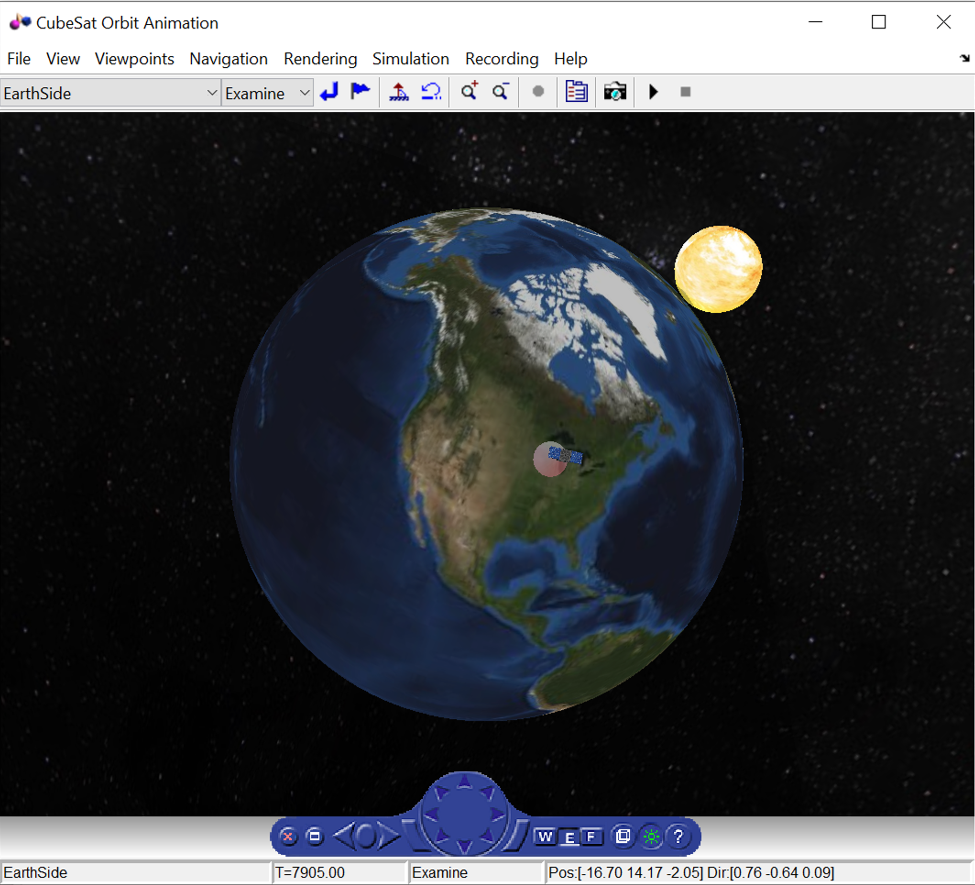
\includegraphics[width=.7\textwidth]{Fig/CubeSatModelScreenshot.png}
\caption{A screen capture of the CubeSat Orbit Animation window from the Aerospace Blockset CubeSat Simulation Library. This image shows the CubeSat within line-of-sight of the proscribed virtual ground station located in Ames, Iowa.}
\label{OrbitalAnimation}
\end{figure}
%%%%%%%%%%%%%%%%%%%%%%%%%%%%%%%%%%%%%%%%%%%%%%%%%%%%%%%%%%%%%%%%%%%%%%%%%%%%%
%%%%%%%%%%%%%%%%%%%%%%%%%%%%%%%%%%%%%%%%%%%%%%%%%%%%%%%%%%%%%%%%%%%%%%%%%%%%%

The values we use for the orbital simulation are shown in Table \ref{OrbitalParameters}. %\textcolor{blue}{Try to rotate the table and minimize the free space}.
The simulation time is chosen to be one week in order to provide a decently long%"decently long" doesn't feel like a super technical/professional phrase; consider rewording
time interval with many orbital passes, while also being reasonable for computation time. All values shown in this table are selected based upon the expected orbital parameters of ISU's first CubeSat mission, CySat \cite{Nelson2020}. This upcoming mission will be deployed via the nanoracks system on-board the International Space Station (ISS), so the orbital parameters are very close to those of the ISS. This portion of the model serves to provide us with orbital information of a user-defined CubeSat mission rather than building and launching a physical craft. It is important to note that any Earth-orbiting CubeSat orbit %Earth-orbiting CubeSat orbit is redundant
could be defined for this project, provided that orbit brings the craft within line-of-sight of the virtual ground station at some point in time during the simulation. 

The positions and velocities of the CubeSat calculated in the orbital simulation allow for imitating its interaction with a virtual ground station. We choose the location of the ground station to be at a latitude of 42.0236$^{\circ}$N and a longitude of -93.6528$^{\circ}$W as described in Table \ref{OrbitalDatasets} in the Appendix. These parameters correspond to expected values for the CySat mission, which will use a real ground station at these coordinates to download data from the satellite \cite{Nelson2020}. We also note that the simulation assumes sea-level altitude for the ground station's position, and does not include topographical differences that might be present if the ground station location were to be changed.

We next use output from the orbital simulation blocks along with the ground station position to determine if line-of-sight (LOS) between the CubeSat and ground station is achieved at each time step. Using the satellite position vector, and ground station position, we calculate the azimuth and elevation of the CubeSat with respect to the ground station. The simulation can then determine whether or not LOS is achieved between the CubeSat and the ground station by monitoring only the calculated elevation angle. Figure \ref{OrbitalDatasets} shows every dataset generated by the orbital simulation, including the number of orbits the CubeSat experiences, a binary representation of the LOS calculation, a binary representation of CubeSat and ground station connection, simulated received bits with the specified baud rate, and the azimuth and elevation angles of the CubeSat.

The system variables referring to all of the datasets in Figure \ref{OrbitalDatasets} are shown in Table \ref{GroundStationVariables}. We refer to these variables throughout the rest of the paper, when describing the formal specifications written for each as well as in analyzing the RV output.

%%%%%%%%%%%%%%%%%%%%%%%%%%%%%%%%%%%%%%%%%%%%%%%%%%%%%%%%%%%%%%%%%%%%%%%%%%%%%
%%%%%%%%%%%%%%%%%%%%%%%%%%%%%%%%%%%%%%%%%%%%%%%%%%%%%%%%%%%%%%%%%%%%%%%%%%%%%
\begin{figure}[!ht]
\centering
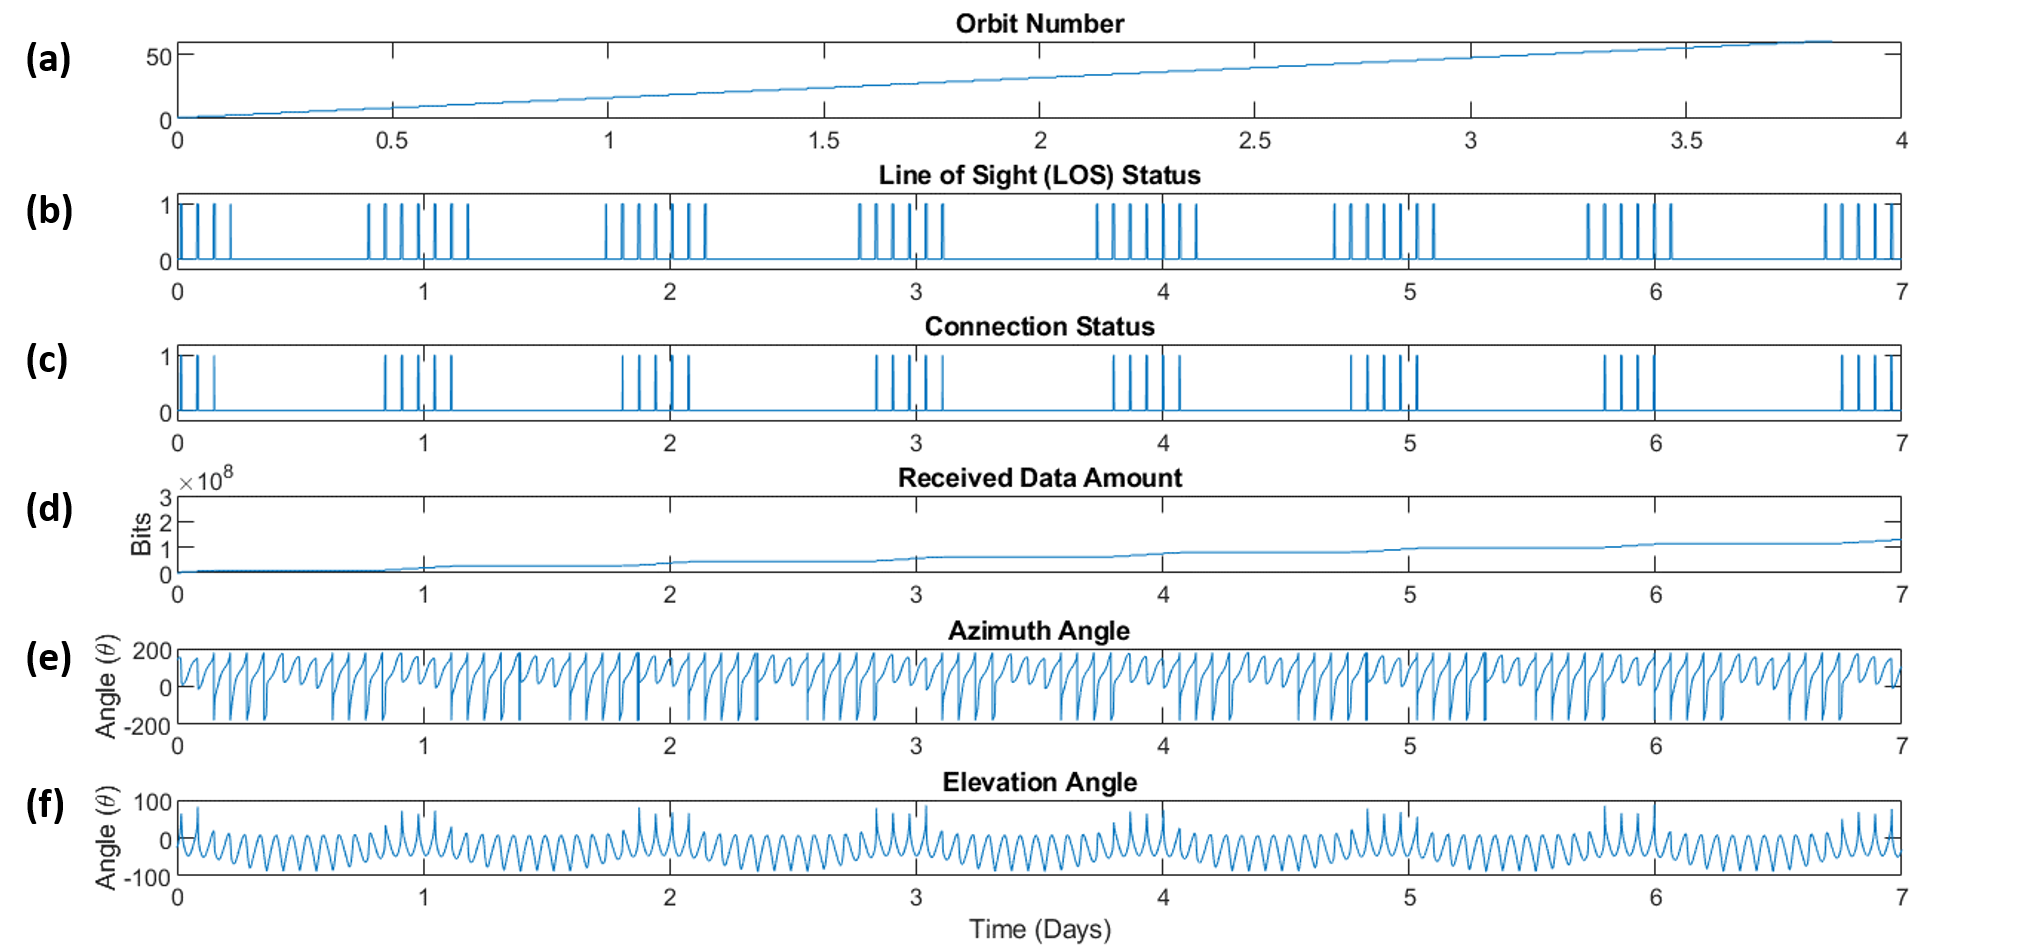
\includegraphics[width=1\textwidth]{Fig/OrbitSimulationDataUpdated5.png}
\caption{Datasets recorded during the orbital simulation. (a) The orbit number of the CubeSat throughout the simulation. (b) Binary representation of when line-of-sight (LOS) is achieved between the CubeSat and the ground station. (c) Binary representation of when the signal-to-noise ratio (SNR) is great enough during LOS that communication between the CubeSat and ground station is possible. (d) Estimated number of bits received by the ground station with a 9600 baud rate. (e) Azimuth angle of the CubeSat with respect to the ground station. (f) Elevation angle of the CubeSat with respect to the ground station.}
\label{OrbitalDatasets}
\end{figure}
%%%%%%%%%%%%%%%%%%%%%%%%%%%%%%%%%%%%%%%%%%%%%%%%%%%%%%%%%%%%%%%%%%%%%%%%%%%%%
%%%%%%%%%%%%%%%%%%%%%%%%%%%%%%%%%%%%%%%%%%%%%%%%%%%%%%%%%%%%%%%%%%%%%%%%%%%%%

\vspace{15 mm}

\begin{table}[!h]
\centering
\begin{tabular}{ll} 
\hline\hline
\textbf{Signal} & \textbf{Description}                               \\ 
\hline
\texttt{Time}            & Number of seconds into simulation.                 \\
\texttt{LOS}             & Line of sight indication.                          \\
\texttt{Conn}            & Connection status indication.                      \\
\texttt{Received}        & Theoretical data downlinked with 9600 baud.        \\
\texttt{OrbitNum}        & Number of orbits since simulation start.           \\
\texttt{Az}              & Azimuth angle of spacecraft wrt ground station.    \\
\texttt{El}              & Elevation angle of spacecraft wrt ground station.  \\
\hline\hline
\end{tabular}
\caption{Variables representing the dataset outputted by the orbital simulation portion of the communications system model.}
\label{GroundStationVariables}
\end{table}

\subsection{Simulated Communicaitons}
\label{ref:comm}

When designing a real CubeSat communications system, developers typically perform link budgeting early to determine several properties in their communications system \cite{daylee2018}. These calculations aid in understanding the gain and power requirements for the transmitting and receiving antennas of the system and are a primary factor in determining what kind of equipment is necessary to build a communication link. Link budgeting is not an exact science, since the main equations assume an ideal system \cite{Zyren1998}, but it is commonly used by CubeSat developers. Because we are simulating a communications system for this case study, we model the antenna directly first and then calculate the link during the simulation.

For the transmitting antenna, we model a microstrip patch antenna using the Mathworks Antenna Toolbox \cite{AntennaToolbox}. This type of antenna is popular with CubeSat developers due to their compact size and efficiency \cite{Tharun2019,Neveu2013,Liu2019}. The ground station antenna parameters are derived from an MSquared 436CP42UG antenna, though in our model this only influences the antenna receiver gain \cite{M2AntennaSystems}. As with the orbital simulation, we choose the parameters for the transmitting antenna used in the simulation based on those of a real antenna on the upcoming CySat mission \cite{Nelson2020}. All parameters for the transmitting antenna, shown in \ref{AntennaParameters}, approximately model this antenna except for the transmitting frequency. The transmission frequency is chosen to be 3.4 GHz in the S-band, which is currently a popular band for developers interested in downlinking relatively large amounts of data \cite{daylee2018,Pittella2016,Nascetti2015,FaiselTubbal2015,Islam2015}. We then produce the antenna's gain pattern in matrix-form outside of the simulation, which is used in determining the link.

During the simulation, the antenna gain pattern is loaded in during the beginning setup. While the orbital simulation of the model progresses, the signal-to-noise ratio (SNR) is calculated at each time step that LOS is achieved. This ratio is calculated using the link equation, which relates all necessary parameters in a communication system including but not limited to: data rate, antenna size, propagation path length, and transmitter power \cite{Wertz1999,IET2014}. The general form of the link equation is shown in Equation \ref{LinkEquation}. A required SNR for the connection is predefined as 3 dB, and communication is considered possible when the calculate SNR is equal to or greater than this threshold. Communication achievement is plotted as a Boolean in Figure \ref{OrbitalDatasets}.c. In addition to communication status, the theoretical amount of data that can be transmitted is also tracked, and is shown in Figure \ref{OrbitalDatasets}.d.
%
\begin{equation}
\frac{E_b}{N_o} = P + G_t + L_{pt} + L_l + L_{pr} + L_s + L_a + G_r + 228.6 - 10 \cdot \log(T_s) - 10 \cdot \log(R)
\label{LinkEquation}
\end{equation}
%\vspace{5 mm}
%
where E$_{b}$/N$_{o}$ is the ratio of received energy per bit to noise-density,
%(EIRP is the effective isotropic radiated power), 
$P$ is the power of the transmitter, $G_t$ is the TX antenna gain, $L_l$ is the transmitter-to-antenna line loss, $L_{pr}$ is the receiving antenna pointing loss, $L_s$ is the space loss, $L_a$ is the propagation and polarization loss, $G_r$ is the RX antenna gain, $T_s$ is the system noise temperature, and $R$ is the data rate of the link \citep{Wertz1999}. The value of $L_s$ changes greatly as the CubeSat orbits, and is therefore an important parameters in this calculation. $L_{pt}$ and $L_{pr}$ also play an important role, since accurate pointing is necessary for directional antennas. The term $L_a$ is a function of factors consisting of atmospheric and precipitation-induced losses, and is assumed to be negligible in the model.

\subsection{Radio Transmission}
\label{ref:radio}

The radio transmission portion of the model can be considered a component of the communications simulation. It uses a Universal Software Radio Peripheral (USRP) B210 software-defined radio (SDR) from Ettus Research to perform quaternary phase-shift keying transmission and reception of sample telemetry data, as if a CubeSat were transmitting to the ground station. This portion of the model is built using the MathWorks Communications Toolbox \cite{CommunicationsToolbox}. Telemetry is broadcasted from the transmitting antenna to the receiving antenna when the communication status, shown in Figure \ref{OrbitalDatasets}.c is active. The transmission takes place specifically at each time step where the communication status goes from inactive to active.

%%%%%%%%%%%%%%%%%%%%%%%%%%%%%%%%%%%%%%%%%%%%%%%%%%%%%%%%%%%%%%%%%%%%%%%%%%%%%
%%%%%%%%%%%%%%%%%%%%%%%%%%%%%%%%%%%%%%%%%%%%%%%%%%%%%%%%%%%%%%%%%%%%%%%%%%%%%
\begin{figure}[!ht]
\centering

\includegraphics[width=1\textwidth]{Fig/SampleTelemetry.png}
\caption{A sample of the simplified telemetry messages that are broadcasted in the communications model. This information is contained within a file. Each parameter listed in the telemetry is a typical piece of information that could be collected in a real CubeSat mission.}
\label{SampleTelemetry}
\end{figure}
%%%%%%%%%%%%%%%%%%%%%%%%%%%%%%%%%%%%%%%%%%%%%%%%%%%%%%%%%%%%%%%%%%%%%%%%%%%%%
%%%%%%%%%%%%%%%%%%%%%%%%%%%%%%%%%%%%%%%%%%%%%%%%%%%%%%%%%%%%%%%%%%%%%%%%%%%%%

Each transmission consists of a sample telemetry dataset contained within a file. The telemetry message is comprised of a handful of parameters relating to the operation of a CubeSat's on-board communications system that would be of interest during a real mission. A sample telemetry message that is broadcasted in this model is shown in Figure \ref{SampleTelemetry}. This sample message is a simplified version of a typical CubeSat telemetry message, which may consist of hundreds of parameters covering all CubeSat systems. Using a larger message is possible with the configuration we have developed, but for the sake of simplicity, we maintain a small set of values in the message.

%%%%%%%%%%%%%%%%%%%%%%%%%%%%%%%%%%%%%%%%%%%%%%%%%%%%%%%%%%%%%%%%%%%%%%%%%%%%%
%%%%%%%%%%%%%%%%%%%%%%%%%%%%%%%%%%%%%%%%%%%%%%%%%%%%%%%%%%%%%%%%%%%%%%%%%%%%%
\begin{figure}[!h]
\centering
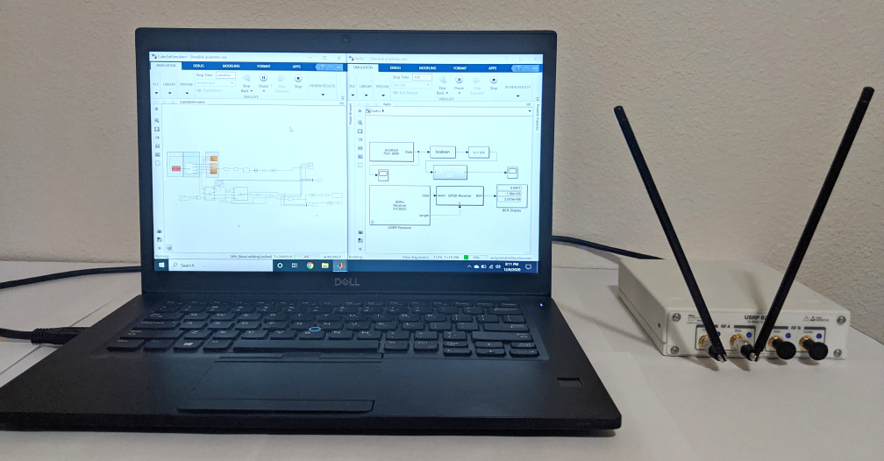
\includegraphics[width=1\textwidth]{Fig/Hardware.png}
\caption{The test setup used in this case study. A Dell Latitude 7490 is used for running the communication simulation. A Universal Software Radio Peripheral (USRP) B210 Software Defined Radio (SDR) performs the communication between ANT500 telescopic transmitting and receiving antennas.}
\label{Hardware}
\end{figure}
%%%%%%%%%%%%%%%%%%%%%%%%%%%%%%%%%%%%%%%%%%%%%%%%%%%%%%%%%%%%%%%%%%%%%%%%%%%%%
%%%%%%%%%%%%%%%%%%%%%%%%%%%%%%%%%%%%%%%%%%%%%%%%%%%%%%%%%%%%%%%%%%%%%%%%%%%%%

When the communications simulation indicates transmission is active, this telemetry message is read into the model and encoded into bits, preceded by a unipolar Barker code \cite{Barker1953,Soba2013}. The message then goes through quadrature phase shift keying (QPSK) modulation with a $\pi$/4 phase offset. The signal is sent through a raised cosine transmit filter, which upsamples and filters the input signal to prepare it for transmission. This signal is then sent to the Universal Software Radio Peripheral (USRP) B210 SDR and transmitted at 3.4 GHz; the same frequency used in the model. The receiver, which is constantly listening for a signal throughout the simulation period, acquires the transmitted waveform and processes it through a similar demodulation process and a data decoder.
%an automatic gain controller (AGC), a raised cosine receive filter, a coarse frequency compensator, symbol and carrier synchronizers, a preamble detector, a frame synchronizer, and finally a data decoder.
This decoder outputs the telemetry message, which is then organized into a comma-separated variable (CSV) file for later use. Each transmission that is received is appended to this file, generating a collection of telemetry messages received throughout the simulation. The system variables referring to all of the datasets in Figure \ref{SampleTelemetry} are shown in Table \ref{CubeSatVariables}. We refer to these variables throughout the rest of the paper, when describing the formal specifications written for each as well as in analyzing the RV output.\\

\begin{table}[!h]
\centering
\begin{tabular}{ll} 
\hline\hline
\textbf{Signal} & \textbf{Description}                     \\ 
\hline
\texttt{Beacon}          & Identifier                               \\
\texttt{Type}            & Identifier                               \\
\texttt{ID}              & Identifier                               \\
\texttt{Score}           & Identifier                               \\
\texttt{Radio\_3V3\_C}   & 3V3 line current to radio.               \\
\texttt{Radio\_3V3\_V}   & 3V3 line voltage to radio.               \\
\texttt{Radio\_VBATT\_C} & Current to radio battery.                \\
\texttt{Radio\_VBATT\_V} & Voltage to radio battery.                \\
\texttt{Radio\_RX}       & Number of radio receptions.              \\
\texttt{Radio\_TX}       & Number of radio transmissions.           \\
\texttt{Radio\_Temp}     & Temperature of radio.                    \\
\texttt{Radio\_PA\_Temp} & Temperature of radio power amplifier.    \\
\texttt{Op\_Count}       & Number of operations perfomed by radio.  \\
\texttt{RSSI}            & Received signal strength indicator.      \\
\hline\hline
\end{tabular}
\caption{Variables that make up the sample telemetry that is broadcasted by the radio communications portion of the model.}
\label{CubeSatVariables}
\end{table}

%For a given CubeSat mission, the received telemetry is the crucial bit of information used to determine whether or not the CubeSat is in a healthy state. In order to make that determination, that telemetry needs to be correct. But how do we determine that? How do we keep track of potentially hundreds of system variables in order to understand our system's performance? How can we differentiate between a system failure and a simple bad data collection, or perhaps a bad bit that wasn't communicated correctly? When do we know the information we're receiving is just a false positive or false negative? Without accurate information, we cannot reason about the system to determine its state, and what, if anything, needs to be done to solve the problems it could be facing. In the next section, we implement a methodology using techniques from the field of formal methods that addresses this issue, and evaluates the performance of our communications system model.

%%%%%%%%%%%%%%%%%%%%%
\section{Communications System Runtime Specifications}
%%%%%%%%%%%%%%%%%%%%%

In this section, we discuss both subsystems of our CubeSat communications model and the process for encoding their requirements into temporal logic. Specific challenges with incorporating RV via the R2U2 tool are highlighted. We discuss multiple methods for validating our specifications and point out specific patterns that we observed during their development and testing.

The specifications for the model are written using temporal logic, to clearly define their meaning and prevent misinterpretation \cite{Roz16}. Mission-time Linear Temporal Logic (MLTL) is ideal for describing such a model because it can reason over time \cite{RRS14,LVR19,LR18}. Additionally, MLTL is able to efficiently filter out false positives and false negatives. Specifications written in MLTL possess integer bounds instead of actual time bounds, meaning they reason over a user-defined number of data points instead of all data within some time frame. This unique aspect of MLTL supports writing specifications that are generalized and reusable on other projects. The MLTL language has been used in many industrial project and since 2018 has been an official logic of the Runtime Verification Benchmark Competition \cite{RRS14,GRS14,SRRMMI15,RSI15,SMR15,SMR16,MRS17,RVBC2018}.\\

When writing our specifications, we consider the methodology and specification types discussed in \cite{Roz16} and \cite{Cauwels2020}. These studies highlighted the necessity of classifying specifications according to how they bound the system. For example, a sensor bound specification may say that the azimuth angle of a CubeSat cannot exceed (-180$^{\circ}$, 180$^{\circ}$). Typical CubeSat systems are similar to the unmanned aircraft systems (UAS) described in \cite{Cauwels2020}. Due to limitations with our model, we do not present specifications in the control-sequence and inter-sensor relationship categories, since the orbital simulation and telemetry collections are validated separately.

\subsection{Orbit Specifications}

The orbital simulation possesses very fine detail due to the ordinary differential equation (ODE) solver that is used to run it. Because so many constants and unchanging values are used to define this part of the model, the number of specifications that can be defined is limited. These specifications stem from a basic understanding of how communications systems operate as well as an understanding of spherical geometry. We discuss two of these specifications in-depth. 

Communication between the spacecraft and the ground station can only occur when the spacecraft is above the horizon. If the CubeSat and ground station cannot are not within line-of-sight of each other, then communication cannot occur. Such a situation would be physically impossible, but these bounds are not automatically assumed by a computer. We therefore define this requirement in MLTL, with an atomic proposition indicating the elevation of the CubeSat must be greater than 0. An additional atomic proposition is written when successful communication takes place, indicated when the value of CONN is 1. The full specification, reasoning over the length of the entire CubeSat's mission, is shown in Appendix D, Specification 1. This specification ensures that communication is only taking place when physically possible, and any measurement indicating otherwise would indicate an issue with measuring the position of the craft.

The azimuth angle of the spacecraft must always be bounded between -180$^{\circ}$ and 180$^{\circ}$. This information is easy to understand, considering the conventional spherical coordinate system. It is physically impossible in this coordinate system for a spacecraft to be located at an azimuth angle outside of this range. Any measurement outside of this range would certainly have to be either a bad data point, or the indication that some fault has occurred in the system. It is easy as humans to understand this requirement, but less so for a computer unless properly defined. With MLTL, we can more robustly express this requirement while accounting for the fact that at some point, an off-nominal data point will be measured. An atomic proposition exists for each of the bounds. Finally, we also specify a $\Delta$ value, indicating that the change in the azimuth angle of the spacecraft cannot change by more than 10$^{\circ}$ from the previous time step. If the spacecraft went from an azimuth angle of, say, -90$^{\circ}$ to 90$^{\circ}$ in one second, that would certainly be concerning. A third atomic proposition encodes this requirement. The full specification, reasoning over the length of the entire CubeSat's mission, is shown in Appendix D, Specification 2. A very similar specification is written for the elevation angle, but with different bounds owing to the spherical coordinate system.

In addition to these two specifications, we also describe the bounds of the elevation angle in Appendix D, Specification 3, and a monitor for the number of orbits the CubeSat experiences, in Appendix D, Specification 4. (We additionally wrote a specification to monitor for the amount of theoretically received data, shown in Figure \ref{OrbitalDatasets}.d that is almost identical to Specification 4.

\subsubsection{\textbf{Necessity of Line-of-Sight Communication}}
“Communication between the spacecraft and ground station can only occur when the spacecraft is above the horizon, ie. the elevation angle of the spacecraft must be above 0. (Line of sight conditions are met.)"
\[ Atomic\:Propositions \begin{cases}
  \varphi_1 & (El_{SAT} > 0) \\
  \varphi_2 & CONN == 1) \\
\end{cases} \]
\begin{equation}
    \label{Spec 1}
    G_{[0,M]} \{(G_{[0,3]}(\varphi_2 \rightarrow \varphi_1))\}
\end{equation} 
This specification stems from common sense, as there must be line of sight between the CubeSat and the ground station.

\subsubsection{\textbf{Azimuth Angle Bounds}}
“The azimuth angle of the CubeSat, Az$_{SAT}$, will be bounded by 0 and 360 at all instances. The current value of Az$_{SAT}$ will not vary more than 1$^{\circ}$ from the previous time step."
\[ Atomic\:Propositions \begin{cases}
  \varphi_1 & (Az_{SAT} \geq -180) \\
  \varphi_2 & (Az_{SAT} \leq 180) \\
  \psi & (abs(Az_{SAT} - Az_{SAT(i-1)}) < 1.0) \\
\end{cases} \]
\begin{equation}
    \label{Spec 2}
    G_{[0,M]} \{(G_{[0,3]}(\varphi_1 \wedge \varphi_2 \wedge \psi))\}
\end{equation} 

\subsubsection{\textbf{Elevation Angle Bounds}}
“The elevation angle of the CubeSat, El$_{SAT}$, will be bounded by -90 and 90 at all instances."
\[ Atomic\:Propositions \begin{cases}
  \varphi_1 & (El_{SAT} \geq -90) \\
  \varphi_2 & (El_{SAT} \leq 90) \\
  \psi & (abs(El_{SAT} - El_{SAT(i-1)}) < 1.0) \\
\end{cases} \]
\begin{equation}
    \label{Spec 3}
    G_{[0,M]} \{(\varphi_1 \wedge \varphi_2 \wedge \psi)\}
\end{equation} 

\subsubsection{\textbf{Orbit Number Check}}
“The orbit number of the spacecraft provided by the model will never be less than 0. The orbit number of the current time step will be equal to or greater than the orbit number from the previous time step."
\[ Atomic\:Propositions \begin{cases}
  \varphi_1 & (OrbNum \geq 0) \\
  \psi_1 & (OrbNum \geq OrbNum_{i-1})\\
\end{cases} \]
\begin{equation}
    \label{Spec 4}
    G_{[0,M]} \{(\varphi_1 \wedge \psi_1)\}
\end{equation} 
This information is crucial to knowing how many passes the CubeSat has made, and also acts as a check to ensure the information pulled from the model is sensible.

\subsection{Telemetry Specifications}

Specifications of the telemetry variables are written with bounds commonly used by CubeSat developers. Developers tend to use component specification sheets when testing their systems, and use the bounds described in those sheets for validating their work. Because the data sheet component specifications often end up acting as requirements when testing the CubeSat, the same methods are applied here.%The previous sentence is unclear; it doesn't tell me what exactly you "applied here"

When considering voltage lines powering CubeSat systems, a tolerance of $\pm$10$\%$ is generally accepted. Unless switched into another state, voltage lines commonly remain active during the mission. Therefore, we write the following specification. The radio 3.3V line must not vary more than 10$\%$ from the desired 3.3V value. The upper and lower bounds are each encoded into atomic propositions. We also consider the case where the measured voltage is within these bounds but may experience oscillation. For this reason, a third atomic proposition is written indicating that the voltage measurement must not vary more than .5V from the previous time step. The full specification, reasoning over the length of the entire CubeSat's mission, is shown in Appendix D, Specification 7. Such a specification is useful for any voltage that is measured and added to the telemetry message, and a similar form exists for measured currents and temperatures as well.

The sample telemetry also lists the number of times that the CubeSat's on-board radio has transmitted. This is an interesting piece of information since it alerts ground station operators as to how many times the radio is attempting to communicate, and if whether or not those communications are received. We write the following specification: the number of times the CubeSat transmits to the ground station will be greater than the previous time the transmission was received. This is another situation where common sense is helpful. We know that the transmit count should be higher between one transmission and the next, but we don't necessarily know if that transmission was the next one to be sent. Hence, keeping track of the radio transmit counts sheds light on how often communication occurs. This specification is encoded into a single atomic proposition without a temporal operator, since each successive measurement of the transmit count should be higher. The full specification, reasoning over the length of the entire CubeSat's mission, is shown in Appendix D, Specification 11. Such a specification is useful for understanding the time evolution of CubeSat telemetry, and diagnosing how effective the communications system is.

We have also written specifications for different temperatures of the radio systems, shown in Specifications 5 and 6 in Appendix D. Current variation for the 3.3V source and Battery Voltage are shown in Specifications 8 and 10 in Appendix D. Similar to Specification 11, we also look at the number of operations the CubeSat's radio performs, detailed in Specification 12 in Appendix D.

\subsubsection{\textbf{Radio Temperature Variation}}
“The temperature of the radio, Radio\_PA\_Temp, will not vary more 1$^{\circ}$ from the previous time step."
\[ Atomic\:Propositions \begin{cases}
  \varphi & (abs(Radio\_Temp - Radio\_Temp_{i-1} \leq 1.0)) \\
\end{cases} \]
\begin{equation}
    \label{Spec 5}
    G_{[0,M]} \{(\varphi)\}
\end{equation} 

\subsubsection{\textbf{Radio Power Amplifier Temperature Variation}}
“The temperature of the radio's power amplifier, Radio\_PA\_Temp, will not vary more 1$^{\circ}$ from the previous time step."
\[ Atomic\:Propositions \begin{cases}
  \varphi & (abs(Radio\_PA\_Temp - Radio\_PA\_Temp_{i-1} \leq 1.0)) \\
\end{cases} \]
\begin{equation}
    \label{Spec 6}
    G_{[0,M]} \{(\varphi)\}
\end{equation} 

\subsubsection{\textbf{Radio 3.3V Voltage Variation}}
“The Radio 3.3V line, 3.3VRadioVolt, must not vary more than 10\% from the desired 3.3V value. It must also not vary more than .5V from the previous time step."
\[ Atomic\:Propositions \begin{cases}
  \varphi_1 & (3.3VRadioVolt \geq 2.97V) \\
  \varphi_2 & (3.3VRadioVolt \leq 3.63V) \\
  \psi & (abs(3.3VRadioVolt - 3.3VRadioVolt_{i-1}) < .5)\\
\end{cases} \]
\begin{equation}
    \label{Spec 7}
    G_{[0,M]} \{G_{[0,3]}(\varphi_1 \wedge \varphi_2 \wedge \psi))\}
\end{equation} 

\subsubsection{\textbf{Radio 3.3V Current Variation}}
“The Radio 3.3V line must not have a current, 3.3VRadioCurr, varying more than 5\% from
the desired current value, 3.3VRadioExpCurr. It must also not vary more than .05A from the value of the previous time step."
\[ Atomic\:Propositions \begin{cases}
  \varphi_1 & (3.3VRadioCurr \geq .95*3.3VRadioExpCurr) \\
  \varphi_2 & (3.3VRadioCurr \leq 1.05*3.3VRadioExpCurr) \\
  \psi & (abs(3.3VRadioCurr - 3.3VRadioCurr_{i-1}) \leq .05)\\
\end{cases} \]
\begin{equation}
    \label{Spec 8}
    G_{[0,M]} \{(\varphi_1 \wedge \varphi_2 \wedge \psi)\}
\end{equation} 

\subsubsection{\textbf{Radio VBatt Voltage Variation}}
“The Radio VBatt voltage, RadioVBattVolt, must not vary more than 10\% from the desired 8.3V value. It must also not vary more than .5V from the previous time step."
\[ Atomic\:Propositions \begin{cases}
  \varphi_1 & (RadioVBattVolt \geq 7.47V) \\
  \varphi_2 & (RadioVBattVolt \leq 9.13V) \\
  \psi & (abs(RadioVBattVolt - RadioVBattVolt_{i-1}) < .5)\\
\end{cases} \]
\begin{equation}
    \label{Spec 9}
    G_{[0,M]} \{(\varphi_1 \wedge \varphi_2 \wedge \psi)\}
\end{equation} 

\subsubsection{\textbf{Radio VBatt Current Variation}}
“The Radio VBatt voltage line must not have a current, RadioVBattCurr, varying more than 5\% from the desired current value, RadioVBattCurrExp. It must also not vary more than .05A from the value of the previous time step."
\[ Atomic\:Propositions \begin{cases}
  \varphi_1 & (RadioVBattCurr \geq .95*RadioVBattCurrExp) \\
  \varphi_2 & (RadioVBattCurr \leq 1.05*RadioVBattCurrExp) \\
  \psi & (abs(RadioVBattCurr - RadioVBattCurr_{i-1}) \leq .05)\\
\end{cases} \]
\begin{equation}
    \label{Spec 10}
    G_{[0,M]} \{(\varphi_1 \wedge \varphi_2 \wedge \psi)\}
\end{equation} 

\subsubsection{\textbf{Transmit Count Check}}
“The number of times the CubeSat transmits to the ground station, Radio\_TX, will be greater than the previous time the transmission was received."
\[ Atomic\:Propositions \begin{cases}
  \varphi & (Radio\_TX > Radio\_TX_{i-1})\\
\end{cases} \]
\begin{equation}
    \label{Spec 11}
    G_{[0,M]} \{(\varphi)\}
\end{equation} 

The number won't necessarily be greater by exactly 1, since the ground station could conceivably not receive a transmission.

\subsubsection{\textbf{Operation Count Check}}
“The number of times the CubeSat performs operations, Radio\_Op\_Count, will be greater than the previous time the transmission was received."
\[ Atomic\:Propositions \begin{cases}
  \varphi & (Radio\_Op\_Count > Radio\_Op\_Count_{i-1})\\
\end{cases} \]
\begin{equation}
    \label{Spec 12}
    G_{[0,M]} \{(\varphi)\}
\end{equation} 

The number won't necessarily be greater by exactly 1, since the ground station could conceivably not receive a transmission.

%A specification describes the desired performance of some aspect of a system. Here, we examine the performance of the simulated communications system particularly with aspects involving transmit/receive operations, measurement of parameters during radio operation, and CubeSat communications monitoring. Since specification is the biggest bottleneck in the design of robust embedded systems \cite{Roz17}, and since formal specification can be a very enlightening activity for the system design process, we treat this as an activity unto itself.\\

%There are two sources of data we wish examine. The first is the set of parameters plotted in Figure \ref{OrbitalDatasets}, which tells us when the CubeSat and ground station are in LOS, when they're communicating, how many times they communicate, etc. The second source of data is the CSV file containing the decoded telemetry, which tells us how the CubeSat's systems are performing, the number of the transmission, voltages and currents, etc. For a typical CubeSat mission, specifications would generally be decided upon before the CubeSat is built and launched, based off the needs of the mission. For our case study, the model was developed alongside a set of specifications. However, the telemetry specifications were written post-implementation so that experimentation with different values and parameters could be performed.\\


%The specifications defining system operations are encoded into mission-time linear temporal logic (MLTL).

%For our specifications, we reference previous ground station designs, the NASA standard for satellite systems developed by the Goddard Space Flight Center (GSFC), and in some cases simply apply common sense \cite{choi2017,Asundi2013,Goddard}. The specifications are written using Mission-time Linear Temporal Logic (MLTL) \cite{RRS14,LVR19}. MLTL has been used in many industrial case studies \cite{RRS14,GRS14,SRRMMI15,RSI15,SMR15,SMR16,MRS17}, and was the official logic of the 2018 Runtime Verification Benchmark Competition \cite{RVBC2018}. Many specifications from other case studies, in logics such as MTL \cite{AH90} and STL \cite{MN04}, can be represented in MLTL. We intuitively relate MLTL to LTL and MTL as follows: (1) MLTL formulas are LTL formulas with bounded intervals over temporal operators, and interpreted over finite traces. (2) MLTL formulas are MTL formulas without any unbounded intervals, and interpreted over finite traces.

%First, we examine the operation of the communications system. A specification is often sourced from previous documentation or reasoning about a similar system, but that is not always the case.

\section{Results}

The simulated communications system we have developed for this case study monitors and outputs orbital data and simulated CubeSat telemetry during a weeklong simulation period. In this section, we compare this data offline, apart from the simulation, against the designed MLTL specifications using the R2U2 tool. In particular, we examine the time necessary to locate faults within these datasets, the amount of memory required by the tool while processing, and other additional statistics detailing the resources required to verify system performance. The R2U2 tool is not integrated into the model due to being run offline. Post-simulation, the data is run through a pre-processing layer that maps multiple inputs into a single Boolean atomic input for R2U2, which is described in further detail in \cite{Cauwels2020}. This methodology provides lower precision than embedding the tool but greatly simplifies the verdicts that it returns.

Throughout the duration of this case study, R2U2 was hosted on an Ubuntu 20.04 LTS operating system on an Intel Core i7-6700K CPU with a 4.00 GHz clock and 32GB of RAM. Separate instances of R2U2 were run for the two datasets, independent of one another. To better understand how the specifications are encoded into observation trees for R2U2, see \cite{Cauwels2020,SMR15,SMR16}.

\subsection{Orbital Dataset Verification}

The orbital dataset is collected throughout the simulation. The data file consists of the \textbf{Time} (s), the system's \textbf{Connection} status in Boolean representation, the CubeSat's estimated \textbf{Received} data with a 9600 baud rate measured in bits, the system's \textbf{LOS} status in Boolean representation,	the CubeSat's \textbf{OrbitNumber} measured as an integer, and the \textbf{Azimuth} and \textbf{Elevation} of the CubeSat measured in degrees. In total, there are 604,801 measurements of each of these parameters during the simulation.

%%%%%%%%%%%%%%%%%%%%%%%%%%%%%%%%%%%%%%%%%%%%%%%%%%%%%%%%%%%%%%%%%%%%%%%%%%%%%
%%%%%%%%%%%%%%%%%%%%%%%%%%%%%%%%%%%%%%%%%%%%%%%%%%%%%%%%%%%%%%%%%%%%%%%%%%%%%
\begin{figure}[!ht]
\centering
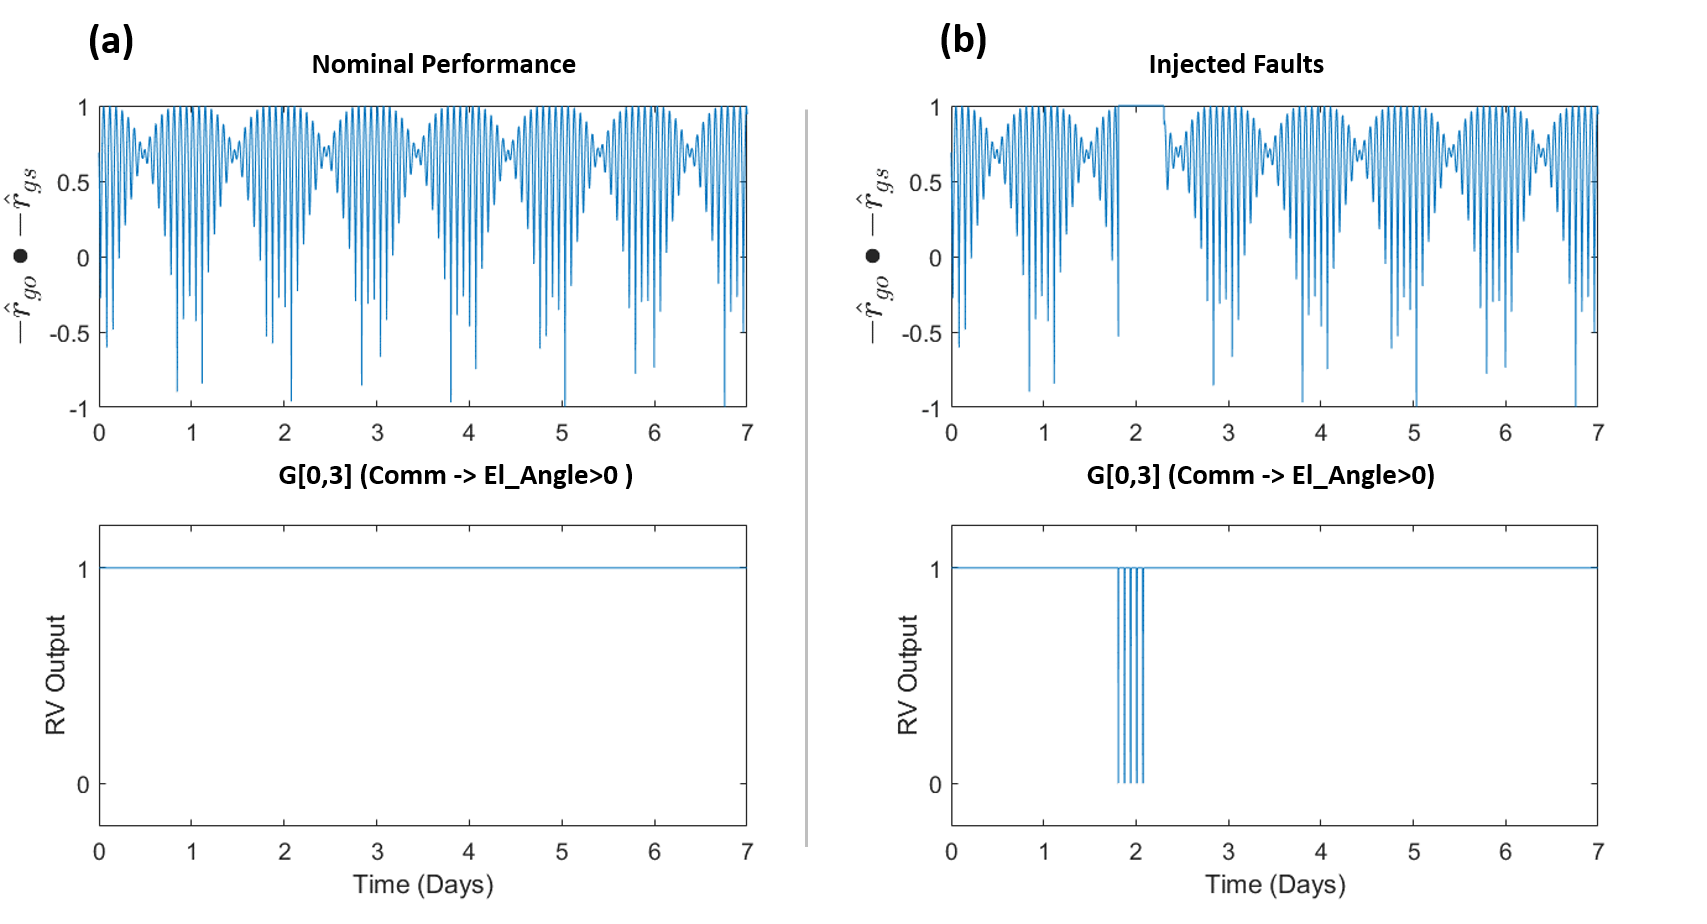
\includegraphics[width=.8\textwidth]{Fig/LOSEL_Spec1.png}
\caption{Results of running Specification 1, titled "Necessity of Line-of-Sight Communication", in R2U2 with multiple datasets. Top plots show a calculated elevation angle of the CubeSat with respect to the ground station. Bottom plots show RV output when the specification is run against the dataset in R2U2. (a) Nominal performance with no change. (b) Injected faults, one during the time of an orbital pass. Temporal operators account for multiple off-nominal measurements before a fault is declared.}
\label{ConnElSpecResults}
\end{figure}
%%%%%%%%%%%%%%%%%%%%%%%%%%%%%%%%%%%%%%%%%%%%%%%%%%%%%%%%%%%%%%%%%%%%%%%%%%%%%
%%%%%%%%%%%%%%%%%%%%%%%%%%%%%%%%%%%%%%%%%%%%%%%%%%%%%%%%%%%%%%%%%%%%%%%%%%%%%

After the simulation is run, we put the orbital data through the pre-processing layer to output a single Boolean atomic input. Using this methodology, we individually validate each of the specifications we have developed for the model. For the orbital simulation, R2U2 monitors and reports if operating ranges, sensor bounds, and rates of change are satisfied for all of the orbital measurements.

Figure \ref{ConnElSpecResults} shows the results for Specification 1 discussed in Section 3 and detailed in Appendix D. The top panels show the elevation angle and CONN status of the CubeSat throughout the simulation, and the bottom panels show the RV output when that data is run through R2U2 with Specification 1. Figure \ref{ConnElSpecResults}.a shows a nominal simulation wherein no faults occur. Figure \ref{ConnElSpecResults}.b shows a simulation with an injected fault in the elevation data, $\sim$3 days into the simulation. R2U2 correctly identifies this fault with our specification.

%%%%%%%%%%%%%%%%%%%%%%%%%%%%%%%%%%%%%%%%%%%%%%%%%%%%%%%%%%%%%%%%%%%%%%%%%%%%%
%%%%%%%%%%%%%%%%%%%%%%%%%%%%%%%%%%%%%%%%%%%%%%%%%%%%%%%%%%%%%%%%%%%%%%%%%%%%%
\begin{figure}[!ht]
\centering
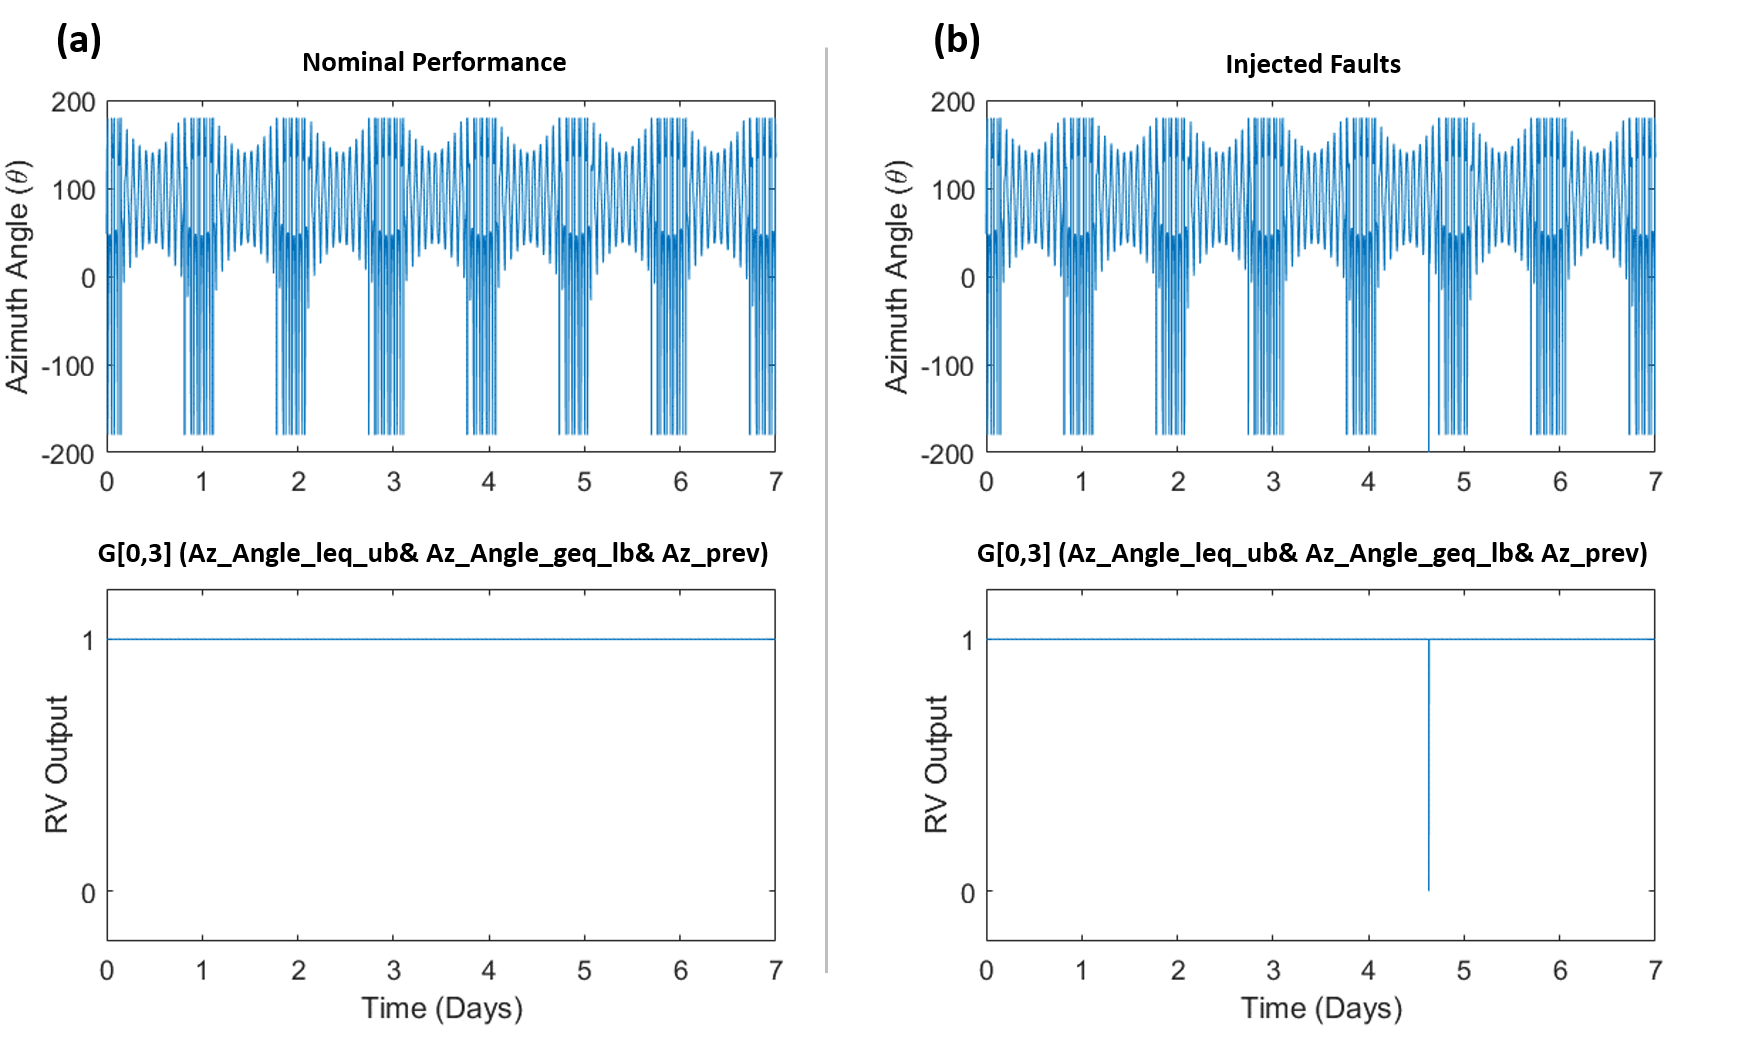
\includegraphics[width=.8\textwidth]{Fig/Az_Spec2.png}
\caption{Results of running Specification 2, titled "Azimuth Angle Bounds", in R2U2 with multiple datasets. (a) Nominal performance with no change. (b) Azimuth data with an injected fault. Temporal operators account for multiple off-nominal measurements before a fault is declared.}
\label{AzAngle}
\end{figure}
%%%%%%%%%%%%%%%%%%%%%%%%%%%%%%%%%%%%%%%%%%%%%%%%%%%%%%%%%%%%%%%%%%%%%%%%%%%%%
%%%%%%%%%%%%%%%%%%%%%%%%%%%%%%%%%%%%%%%%%%%%%%%%%%%%%%%%%%%%%%%%%%%%%%%%%%%%%

Figure \ref{AzAngle} shows the results of Specification 2 discussed in Section 3 and detailed in Appendix D. The top panels show the azimuth angle of the CubeSat throughout the simulation and the bottom panels show the RV output when the data is run through R2U2 with Specification 2. Figure \ref{AzAngle}.a also shows a nominal situation with no faults. Figure \ref{AzAngle}.b shows a simulation with an injected fault in the azimuth data, $\sim$4.5 days into the simulation. R2U2 correctly identifies the fault here as well.

%Using specifications 5,6,7,8,9,10,11 and 12 encoded into MLTL, R2U2 verifies offline that the system is operating nominally for the entire duration within $\sim$ 43 s. This may be considered a non-trivial duration, since that time may be considered too long when deciding whether or not to command the spacecraft during the orbit the most recent telemetry was received. It's of note however that a developer likely wouldn't actively compare the most recent telemetry to the telemetry received during the entire lifetime of the craft, since the computation time for verification would progressively increase to longer and more undesirable durations. However, it would be of benefit to verify a set of the most recently collected telemetry values to monitor for system changes. In this way, we verify the CubeSat's recent performance while saving on computation time. In Figure \ref{OrbitalDataTimes}, we measure the length of time needed to verify progressively longer datasets to measure the efficiency of R2U2's computation power. As Figure \ref{OrbitalDataTimes} shows, this relationship scales linearly (plotted logarithmically for clarity) so the algorithm needed to process this dataset has runtime O(m).\\

\subsection{Telemetry Dataset Verification}

The telemetry data is collected each time the Connection parameter in the orbital simulation goes active. Using the parameters given in Tables \ref{OrbitalParameters},\ref{AntennaParameters}, and \ref{DownlinkParameters} with the simulation results in 46 instances of a virtual connection between the CubeSat and the ground station. The telemetry data consists of a sample set of variables relating to a CubeSat's radio system that would be measured during a real CubeSat mission.

Similar to the orbital dataset, we put the data through a pre-processing layer to output a single Boolean atomic input and individually validate each of the specifications we have developed.

Figure \ref{3V3SpecResults} shows the 3.3V voltage measurement throughout the simulation period. Figure \ref{3V3SpecResults}.a represents a nominal simulation wherein no faults occur. Figure \ref{3V3SpecResults}.b represents a simulation where a few bad data points are collected, but due to the temporal operators of Specification 7, they do not cause a fault. Figure \ref{3V3SpecResults}.c represents a simulation in which a failure takes place and the 3.3V line slowly lowers to 0V. As indicated by the RV output in Figure \ref{3V3SpecResults}.c, a few off-nominal data points are allowed by the temporal operators before declaring a fault has occurred.

%%%%%%%%%%%%%%%%%%%%%%%%%%%%%%%%%%%%%%%%%%%%%%%%%%%%%%%%%%%%%%%%%%%%%%%%%%%%%
%%%%%%%%%%%%%%%%%%%%%%%%%%%%%%%%%%%%%%%%%%%%%%%%%%%%%%%%%%%%%%%%%%%%%%%%%%%%%
\begin{figure}[!ht]
\centering
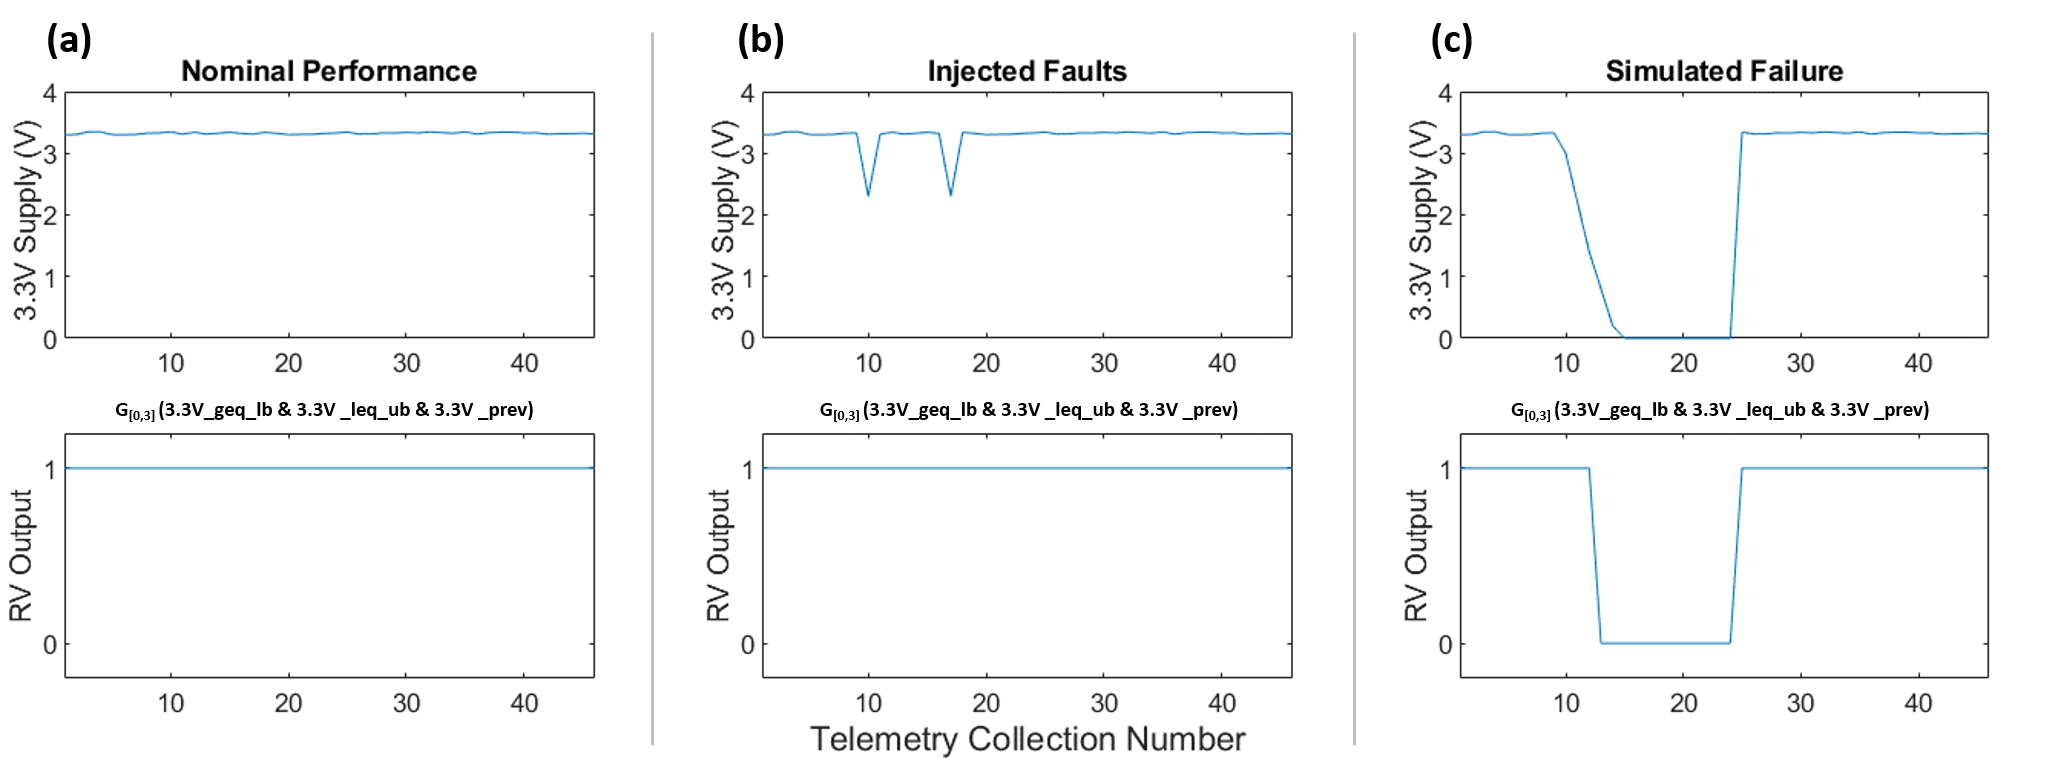
\includegraphics[width=.8\textwidth]{Fig/3V3_Spec7.png}
\caption{Results of running Specification 7, titled "Radio 3.3V Voltage Variation", in R2U2 with multiple datasets. (a) Nominal performance with no change. (b) Multiple injected faults, considered false positives, are accounted for with temporal operators and do not indicate a fault. (c) Simulated failure of voltage supply, fault declared after multiple poor measurements indicates issue.}
\label{3V3SpecResults}
\end{figure}
%%%%%%%%%%%%%%%%%%%%%%%%%%%%%%%%%%%%%%%%%%%%%%%%%%%%%%%%%%%%%%%%%%%%%%%%%%%%%
%%%%%%%%%%%%%%%%%%%%%%%%%%%%%%%%%%%%%%%%%%%%%%%%%%%%%%%%%%%%%%%%%%%%%%%%%%%%%

The 3.3V specification is worth discussing more extensively. Because a CubeSat is a single system composed of multiple subsystems, for a given CubeSat project there could be up to several dozen voltages the developers would want to monitor during the mission phase. Formally specifying these voltages is consistent with the 3.3V voltage monitor described in Specification 7 aside from the bounds assigned to the atomic propositions. This can be seen with Specification 9 in Appendix D, which monitors the 8.3V supplied to the radio's battery. Aside from adjusting the lower and upper bounds, this specification is identical to that of the 3.3V voltage monitor.

Figure \ref{VBATTSpecResults} shows the radio battery voltage measurement throughout the simulation period. Just like with the 3.3V monitor, R2U2 reports if the upper and lower bounds of this voltage parameter are met at each time step. Aside from separate bounds, the specification used to describe this variable is exactly the same as for the 3.3V variable.

%%%%%%%%%%%%%%%%%%%%%%%%%%%%%%%%%%%%%%%%%%%%%%%%%%%%%%%%%%%%%%%%%%%%%%%%%%%%%
%%%%%%%%%%%%%%%%%%%%%%%%%%%%%%%%%%%%%%%%%%%%%%%%%%%%%%%%%%%%%%%%%%%%%%%%%%%%%
\begin{figure}[!hb]
\centering
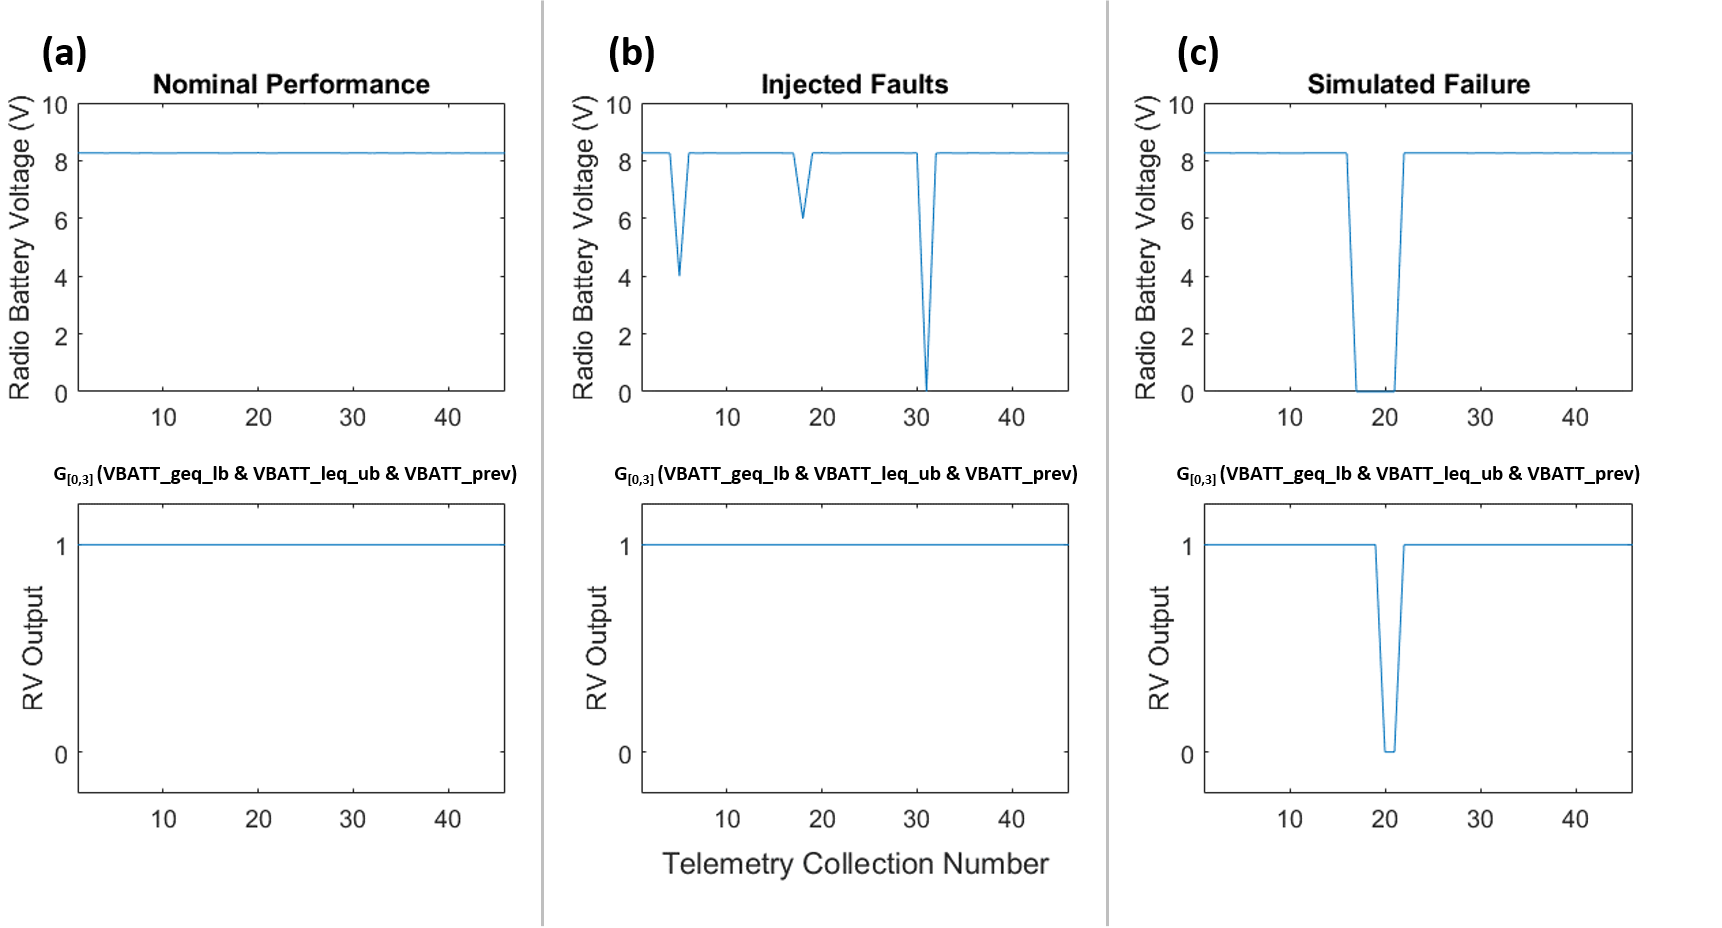
\includegraphics[width=.8\textwidth]{Fig/VBATT_Spec9.png}
\caption{Results of running Specification 9, titled "Radio VBatt Voltage Variation", in R2U2 with multiple datasets. (a) Nominal performance with no change. (b) Multiple injected faults, considered false positives, are accounted for with temporal operators and do not indicate a fault. (c) Simulated failure of voltage supply, fault declared after multiple poor measurements indicates issue.}
\label{VBATTSpecResults}
\end{figure}
%%%%%%%%%%%%%%%%%%%%%%%%%%%%%%%%%%%%%%%%%%%%%%%%%%%%%%%%%%%%%%%%%%%%%%%%%%%%%
%%%%%%%%%%%%%%%%%%%%%%%%%%%%%%%%%%%%%%%%%%%%%%%%%%%%%%%%%%%%%%%%%%%%%%%%%%%%%

%%%%%%%%%%%%%%%%%%%%%
\section{Discussion}
%%%%%%%%%%%%%%%%%%%%%

All but two of the variables comprising the orbital dataset are formally specified, the \texttt{Time} and the \texttt{Received} data. The received data acts as a simple measure of bits%this doesn't feel clear
, but in reality would be much more complex. Because the simulation time is user-defined in our model and is guaranteed to be correct for each time step, there's no utility in defining its operation. With a real-world CubeSat project however, it would be very useful to look at the timestamp at which a certain CubeSat position was recorded, in order to ensure that the desired orbit persists.

In reality, many CubeSat developers extract orbital information about their CubeSats from the gpredict satellite tracking and orbit prediction software \cite{csete2018}. This tool provides an extensive list of parameters for a given satellite or CubeSat that can be used to track its position, determine its velocity, altitude, expected Doppler shift, and more. Collecting all of this information in one location makes the tool popular with developers and amateurs alike. The gpredict tool's calculations for a CubeSat are verified through their own system. If, however, developers wanted to create a separate model of their CubeSat system, then gpredict could be used to verify that the outputs are correct.

There are fourteen separate variables contained within the sample telemetry. Of these, our specifications cover nine. Information such as "\_index", "\_type" and "\_id" are handy identifiers for the telemetry message but do not serve to specify a variable in any way. The purpose of these variables is to identify the telemetry message, and would instead be used to check if the signal is from a specific CubeSat. Formally specifying these variables is possible, but it would likely be just as well to check them with a simple string comparison. The variable "\_score" may either rate the telemetry or indicate what kind of telemetry the specific message is, so we have not explored it here. Finally, we did examine the received signal strength indicator (RSSI) variable "Lithium RSSI", which is a measure of beacon signal strength from the radio receiver. This variable also essentially acts as a rating for the signal, so we have not explored it here.

Without real hardware to test, verification of a CubeSat communications system model presents several difficulties. Many of the results in the simulation are guaranteed to be correct, such as the time the CubeSat is in a given position. We are limited in this respect because timestamps of spacecraft position are examined in practice to ensure they are sensible. Additionally, the telemetry messages that were transmitted and received were not influenced by the system from which they were derived. We have discussed how utilizing COTS components, usually cheaper than the parts used on large-scale spacecraft missions, comes with a trade-off of lower accuracy. Because we developed a model instead of working with actual hardware, we could not account for these problems. To comprehensively explore the verification and validation of a CubeSat communications system, we would develop a real mission like that shown in Figure \ref{CubeSatRVDiagram} and integrate RV into the ground station portion to validate orbital data and information sourced from the CubeSat.

%%%%%%%%%%%%%%%%%%%%%%%%%%%%%%%%%%%%%%%%%%%%%%%%%%%%%%%%%%%%%%%%%%%%%%%%%%%%%
%%%%%%%%%%%%%%%%%%%%%%%%%%%%%%%%%%%%%%%%%%%%%%%%%%%%%%%%%%%%%%%%%%%%%%%%%%%%%
\begin{figure}[!ht]
\centering
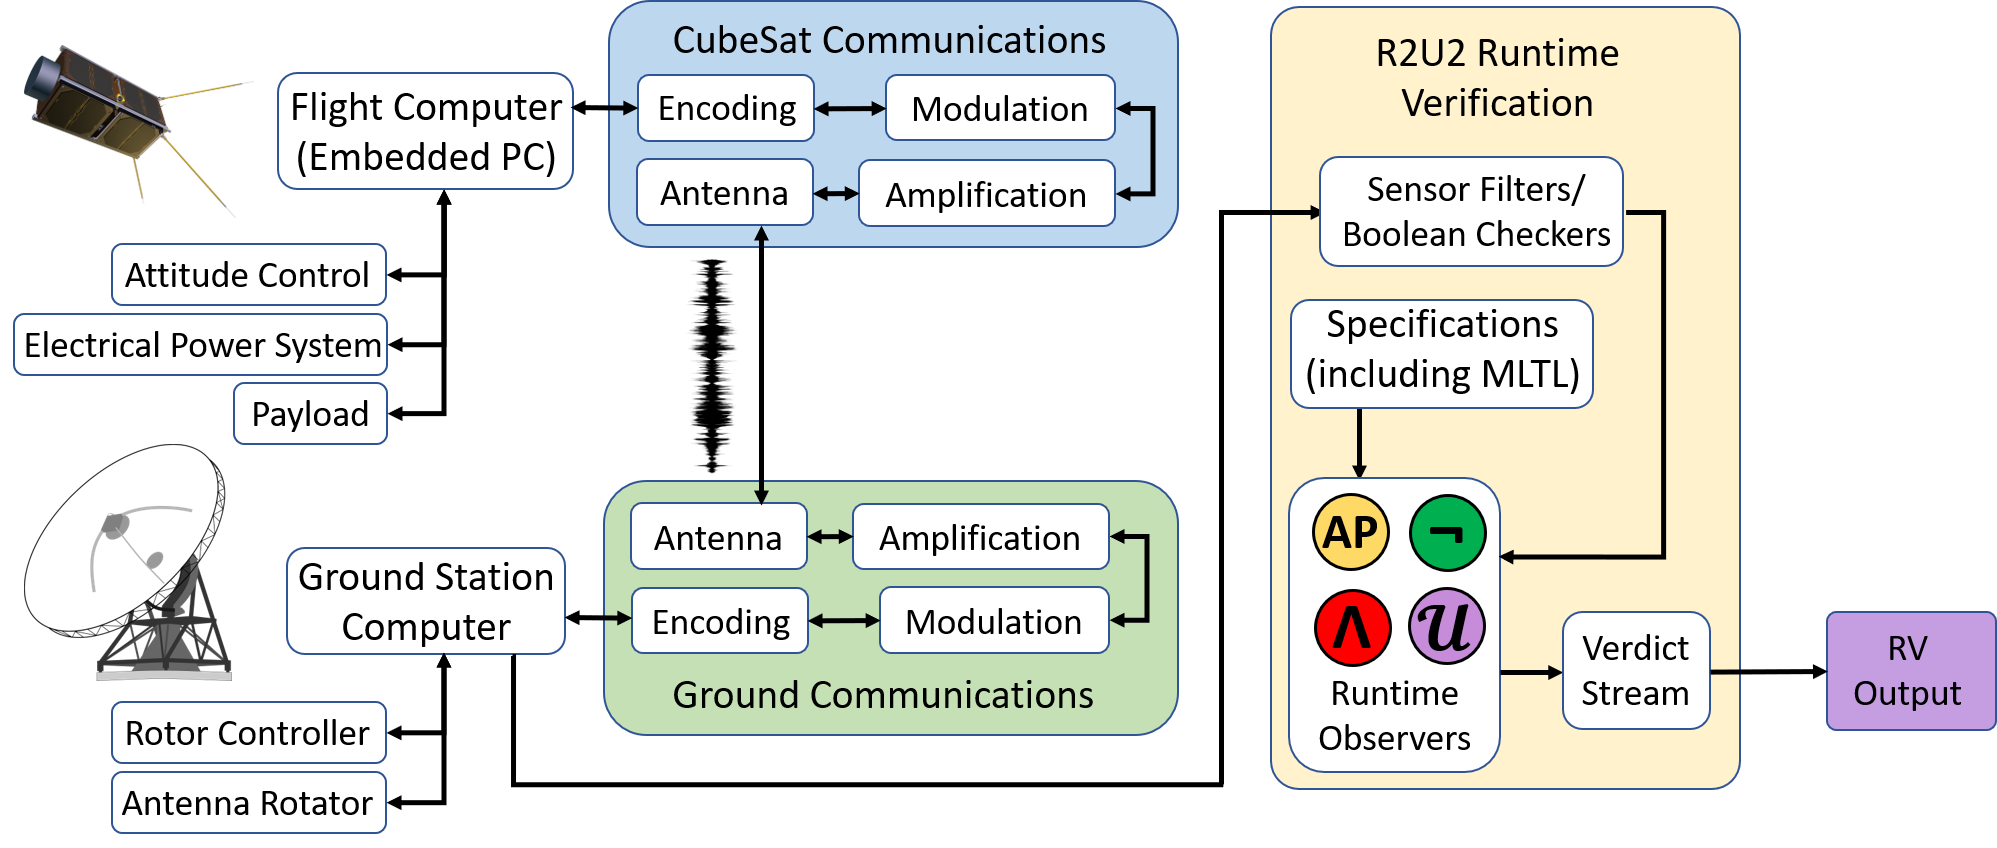
\includegraphics[width=1\textwidth]{Fig/InFlight_Overview.png}
\caption{A representation of how runtime verification fits into a real CubeSat mission's communications system. The CubeSat measures system values and saves them for transmission. The telemetry information is then encoded, modulated, amplified and downlinked to the ground station. After a similar decoding process, the telemetry variables are checked against their specifications using the R2U2 tool. For an actual mission, this would consist of an online process wherein R2U2 is run each time the ground station receives a new set of telemetry. The communications system portion references \cite{Asundi2013} and the runtime verification section is derived from \cite{ARS17}.}
\label{CubeSatRVDiagram}
\end{figure}
%%%%%%%%%%%%%%%%%%%%%%%%%%%%%%%%%%%%%%%%%%%%%%%%%%%%%%%%%%%%%%%%%%%%%%%%%%%%%
%%%%%%%%%%%%%%%%%%%%%%%%%%%%%%%%%%%%%%%%%%%%%%%%%%%%%%%%%%%%%%%%%%%%%%%%%%%%%

CubeSats are systems comprised of multiple subsystems, and the chance of an incorrect measurement or bad transfer of data through the systems is a real possibility. In order to ensure that CubeSat systems are operating correctly, it is essential to check that the data measured in the telemetry meets requirements. We have performed introductory exploration of this for a sample set of telemetry values, but did not examine an entire telemetry dataset. As pointed out in Section 3, the specification for a line voltage (3.3V) is all but identical to the specification for another system voltage (VBATT). While system states need to be taken into account,%the first and second half of this sentence don't go together
we could use this method for formally specifying every system voltage contained within a CubeSat telemetry dataset. We plan to explore this further in future work.

While we have discussed implementing RV into a CubeSat communications system to verify orbital information and sample telemetry, a case could be made to verify all of the telemetry measurements prior to communicating them to a ground station. More specifically, RV could be embedded into the CubeSat flight computer so that all of the measurements contained within the telemetry are validated by the CubeSat itself. The ability to have the CubeSat validate its own systems would remove the need to send detailed telemetry messages, replaced instead with simple verdicts of each subsystem. Implementing this functionality into a CubeSat would mean fewer resources are used to communicate system health to the ground station, and would instead be available to transmit payload data. We will explore this idea as well in future work.


%%%%%%%%%%%%%%%%%%%%%
\section{Conclusion}
%%%%%%%%%%%%%%%%%%%%%

The popularity of CubeSat projects is only expected to grow in the coming years, due mainly to their low cost and fast turnaround times. However, without addressing the high rate of failure of these projects, the common problems faced by developers will persist. Communications system failures have been described as one of the most common issues experienced in CubeSat projects, and such failures often lead to premature mission end. To aid in improved reliability of CubeSat communications systems, we have integrated the R2U2 runtime verification tool into two separate layers of the system: one within a ground station layer to monitor the CubeSat's orbit and connection, and one to monitor the CubeSat's telemetry. We provide a small reference set of specifications for these two separate aspects of the communications system, demonstrating their correctness by validating the model's system parameters offline. While we were limited by the model developed for this case study, we discuss how our work could be expanded for a real CubeSat mission.

%%%%%%%%%%%%%%%%%%%%%
\bibliography{References}
%%%%%%%%%%%%%%%%%%%%%

%%%%%%%%%%%%%%%%%%%%%
\newpage
\section*{Appendix}
%%%%%%%%%%%%%%%%%%%%%%%%%%%%%%%%%%%%%%%%%%%%%%%%%%%%%%%%%%%%%%%%%%%%%%%%%%%%%%%%
%This section contains all of the appendices included in the manuscript.

\subsection{Orbital Simulation Data Values}

\begin{table}[!h]
\centering
\begin{tabular}{|l|l|}
\hline
\textbf{Parameter}         & \textbf{Value} \\ \hline
Radius of Earth (km)       & 6378.137       \\ \hline
Avg. Radius of Orbit (km)  & 7078.137       \\ \hline
Eccentricity               & 0              \\ \hline
Inclination (deg)          & 51.6           \\ \hline
RA of Ascending Node (deg) & 0              \\ \hline
Argument of Perigee (deg)  & 0              \\ \hline
True Anomaly (deg)         & 0              \\ \hline
GS Latitude (deg)          & 42.0236        \\ \hline
GS Longitude (deg)         & -93.6528       \\ \hline
\end{tabular}
\vspace{2 mm}
\caption{Parameters of the simulated CubeSat orbit and location of ground station.}
\label{OrbitalParameters}
\end{table}

\subsection{Antenna Design Parameters}

\begin{table}[!h]
\centering
\begin{tabular}{|l|l|}
\hline
\textbf{Parameter}          & \textbf{Value}                      \\ \hline
Length (m)                  & 0.0397                              \\ \hline
Width (m)                   & 0.0397                              \\ \hline
Strip Line Width (m)          & 0.0025                              \\ \hline
Notch Length (m)             & 0.0059                              \\ \hline
Notch Width (m)              & 0.0044                              \\ \hline
Patch Center {[}m,m,m{]}     & {[}0,0,0{]}                         \\ \hline
Feed Location {[}m,m,m{]}    & {[}-0.0441,0,0.0022{]}              \\ \hline
Height(m)                   & 0.0022                              \\ \hline
Ground Plane Length (m)       & 0.0882                              \\ \hline
Ground Plane Width (m)        & 0.0882                              \\ \hline
Patch Center Offset {[}m,m{]} & {[}0,0{]}                           \\ \hline
Feed Offset {[}m,m{]}        & {[}-0.0441,0{]}                     \\ \hline
Substrate                   & 1x1 dielectric {[}default values{]} \\ \hline
Substrate Thickness (m)                   & 0.00220435630882353 \\ \hline
Tilt                        & 0                                   \\ \hline
Tilt Axis                    & {[}1,0,0{]}                         \\ \hline
\end{tabular}
\vspace{2 mm}
\caption{Design Parameters of the Microstrip Patch Antenna used in developing the communications system model.}
\label{AntennaParameters}
\end{table}

\clearpage

\subsection{Downlink Constant Values}

\begin{table}[!ht]
\centering
\begin{tabular}{|l|l|}
\hline
\textbf{Parameter}      & \textbf{Value}            \\ \hline
frequency (Hz)          & 3.4*10\textasciicircum{}9 \\ \hline
Aperture Efficiency     & 0.0                       \\ \hline
TX Power (W)            & 10.0                      \\ \hline
TX Line Loss (dB)       & 0.0                       \\ \hline
Sky Temperature (K)      & 290                       \\ \hline
Polarization Loss (dB)   & 3.0                       \\ \hline
Pointing Error Loss (dB)  & 3.0                       \\ \hline
LNA Gain (dB)           & 16.0                      \\ \hline
LNA Noise Figure (dB)   & 1.5                       \\ \hline
RX Line Loss (dB)       & 3.0                       \\ \hline
Radio Noise Figure (dB) & 10.0                      \\ \hline
RX Antenna Gain (dB)    & 18.9                      \\ \hline
R (baud)                & 9600                      \\ \hline
Eb\_N0\_required (dB)   & 10                        \\ \hline
\end{tabular}
\vspace{2 mm}
\caption{Constant values used in the link budgeting step of the model.}
\label{DownlinkParameters}
\end{table}


\begin{comment}
\subsection{Sample Telemetry}

\begin{lstlisting}
{"_index":"Cube_beacon_01","_type":"_doc","_source":{"3.3V Bus Current":0.203,"3.3V Bus Voltage":3.299,"3.3V Input Current":0.105,"5V Bus Current":0.046,"5V Bus Voltage":5.00388,"5V Input Current":0.05,"@timestamp":"2020-01-16T20:46:20Z","ADC curr (?)":0.013250000000000001,"ADCS 3v3 current":-0.21858590000000003,"ADCS 3v3 voltage":3.288,"ADCS 5V current":-0.13066846000000001, "ADCS 5V voltage":4.9730099999999995,"ADCS Temp 0":22.942298435035127,"ADCS Temp 1":22.00006472534369,"ADCS VBatt current":-0.12939579999999998,"ADCS VBatt voltage":8.2126,"Battery Bus Current":0.067,"Battery Bus Voltage":8.2566,"Battery Current":0.16800000000000015,"Battery Temperature":14.91022252000002,"Battery Voltage":8.2698,"Channel 1 board temperature":20.37117822674668,"Channel 1 module temperature":20.28539843309295,"Channel 1 output current":0.004,"Channel 1 output voltage":0.0484,"Channel 1 panel current A":0.0008,"Channel 1 panel current B":0.0008,"Channel 1 panel voltage A":0.023960000000000002,"Channel 1 panel voltage B":0.023960000000000002,"Channel 2 board temperature":20.88575416931667,"Channel 2 module temperature":21.057240334344215,"Channel 2 output current":0.09,"Channel 2 output voltage":8.525,"Channel 2 panel current A":0.0158,"Channel 2 panel current B":0.0414,"Channel 2 panel voltage A":15.693800000000001,"Channel 2 panel voltage B":15.65786,"Channel 3 board temperature":21.742989427224302,"Channel 3 module temperature":22.085746726947946,"Channel 3 output current":0.161,"Channel 3 output voltage":8.551400000000001,"Channel 3 panel current A":0.1308,"Channel 3 panel current B":0.15200000000000002,"Channel 3 panel voltage A":12.189650000000002,"Channel 3 panel voltage B":1.60532,"Channel 4 board temperature":20.800003748429162,"Channel 4 module temperature":21.571581475708626,"Channel 4 output current":0.029,"Channel 4 output voltage":8.5008,"Channel 4 panel current A":0.022000000000000002,"Channel 4 panel current B":0.15500000000000003,"Channel 4 panel voltage A":15.6339,"Channel 4 panel voltage B":1.58735,"Channel 5 Module input voltage":5.106,"Channel 5 board temperature":24.140652432542993,"Channel 5 module temperature":24.48286419790361,"Channel 5 output current":0.007,"Channel 5 panel current A":0.0018,"Channel 5 panel current B":0.001,"Channel 6 Module input voltage":3.7,"Channel 6 board temperature":25.594515948494973,"Channel 6 module temperature":26.70534858484052,"Channel 6 output current":0.129,"Channel 6 panel current A":0.2884,"Channel 6 panel current B":0.013400000000000002,"Datamnt Usage":0.434,"EIMU current":0.00555,"EPS 3.3 Voltage":3.296,"EPS 3.3V Current":0.009800000000000001,"EPS 5V Current":0.0077,"EPS 5V Voltage":4.98477,"FCPU 3V3 Current":0.16869099999999998,"FCPU 3V3 Voltage":3.302,"FCPU Processor Temp":23.541594667502068,"FCPU Var 1":0,"FCPU Var 2":0,"FCPU Var 3":0,"FCPU Var 4":0,"FCPU Var 5":0,"FCPU Var 6":0,"Ioe States":237,"LI 3V3 Current":0.40367200000000003,"LI 3V3 Voltage":3.302,"LI VBATT Current":-0.19264799999999999,"LI VBATT Voltage":8.243400000000001,"Lithium #RX":0,"Lithium #TX":261648,"Lithium MSP430 Temp":0,"Lithium Op Count":11731,"Lithium PA Temp":22.85666520419977,"Lithium RSSI":97,"NumResets":548, "5VSbVolt":5.1200,"5VSbCurr":.0008,"3.3VSbVolt":3.3160,"3.3VSbCurr":.0005,"1.5VSbVolt"1.4930,"1.5VSbCurr":.0004,"Operation Mode":0,"Output Regulator Temperature":24.662146180000008,"PIM 3v3 current":-0.129,"PIM 3v3 voltage":0,"PIM VBatt monitor":0,"RTC Unix Time":1579207577,"SD Usage":0,"SD V (?)":0,"STAMP GPIO States":29809,"TBEx Payload Current":-0.227,"TBEx Payload Voltage":0,"avgNumActiveTasks1":1.64,"avgNumActiveTasks15":1.81,"avgNumActiveTasks5":1.82,"data_checksum_passed":true,"flag":3,"freeMemPlusCache":107632,"header_checksum_passed":true,"pid":0,"sid":83,"telemetry_archive":false,"telemetry_archive_file_num":0,"totNumProcesses":41,"usedMemMinusCache":19272}}
\end{lstlisting}

\end{comment}

\subsection{Ground Station Variables}

\begin{table}[!h]
\centering
\begin{tabular}{ll} 
\hline\hline
\textbf{Signal} & \textbf{Description}                               \\ 
\hline
\texttt{Time}            & Number of seconds into simulation.                 \\
\texttt{LOS}             & Line of sight indication.                          \\
\texttt{Conn}            & Connection status indication.                      \\
\texttt{Received}        & Theoretical data downlinked with 9600 baud.        \\
\texttt{OrbitNum}        & Number of orbits since simulation start.           \\
\texttt{Az}              & Azimuth angle of spacecraft wrt ground station.    \\
\texttt{El}              & Elevation angle of spacecraft wrt ground station.  \\
\hline\hline
\end{tabular}
\end{table}

\subsection{CubeSat Telemetry Variables}

\begin{table}[!h]
\centering
\begin{tabular}{ll} 
\hline\hline
\textbf{Signal} & \textbf{Description}                     \\ 
\hline
\texttt{Beacon}          & Identifier                               \\
\texttt{Type}            & Identifier                               \\
\texttt{ID}              & Identifier                               \\
\texttt{Score}           & Identifier                               \\
\texttt{Radio\_3V3\_C}   & 3V3 line current to radio.               \\
\texttt{Radio\_3V3\_V}   & 3V3 line voltage to radio.               \\
\texttt{Radio\_VBATT\_C} & Current to radio battery.                \\
\texttt{Radio\_VBATT\_V} & Voltage to radio battery.                \\
\texttt{Radio\_RX}       & Number of radio receptions.              \\
\texttt{Radio\_TX}       & Number of radio transmissions.           \\
\texttt{Radio\_Temp}     & Temperature of radio.                    \\
\texttt{Radio\_PA\_Temp} & Temperature of radio power amplifier.    \\
\texttt{Op\_Count}       & Number of operations perfomed by radio.  \\
\texttt{RSSI}            & Received signal strength indicator.      \\
\hline\hline
\end{tabular}
\end{table}

\subsection{Sample Telemetry}

\begin{lstlisting}
{{"_index":"beacon_0_82","_type":"_doc","_id":"fc5d6f47-81f0-5a83-abe9-7b2f21e24c5a","_score":1,"_source":{"LI 3V3 Current":0.22943999999999998,"LI 3V3 Voltage":3.316,"LI VBATT Current":-0.19289599999999998,"LI VBATT Voltage":8.2698,"Lithium #RX":0,"Lithium #TX":173484,"Lithium MSP430 Temp":0,"Lithium Op Count":7911,"Lithium PA Temp":16.764199712583377,"Lithium RSSI":106}}}
\end{lstlisting}

\subsection{Sample Specifications for the Modeled CubeSat Communications System}

This appendix consists of 12 separate specifications that were developed for this case study. Each specification, written in MLTL, mathematically describes the expected behavior of system variables while removing potential risk of misinterpretation.

\subsubsection{\textbf{Necessity of Line-of-Sight Communication}}
“Communication between the spacecraft and ground station can only occur when the spacecraft is above the horizon, ie. the elevation angle of the spacecraft must be above 0. (Line of sight conditions are met.)"\\
\[ Atomic\:Propositions \begin{cases}
  \varphi_1 & (El_{SAT} > 0) \\
  \varphi_2 & COMM == 1) \\
\end{cases} \]
\begin{equation}
    \label{Spec 1}
    G_{[0,M]} \{(\varphi_2 \rightarrow \varphi_1)\}
\end{equation} \\
This specification stems from common sense, as there must be line of sight between the CubeSat and the ground station.

\subsubsection{\textbf{Azimuth Angle Bounds}}
“The azimuth angle of the CubeSat, Az$_{SAT}$, will be bounded by 0 and 360 at all instances. The current value of Az$_{SAT}$ will not vary more than 1$^{\circ}$ from the previous time step."\\
\[ Atomic\:Propositions \begin{cases}
  $\varphi_1$ & ($Az_{SAT}$ $\geq$ -180) \\
  $\varphi_2$ & ($Az_{SAT}$ $\leq$ 180) \\
  \psi & (abs(Az_{SAT} - Az_{SAT}_{i-1}) < 1.0) \\
\end{cases} \]
\begin{equation}
    \label{Spec 1}
    G_{[0,M]} \{(\varphi_1 \wedge \varphi_2 \wedge \psi)\}
\end{equation} \\

\subsubsection{\textbf{Elevation Angle Bounds}}
“The elevation angle of the CubeSat, El$_{SAT}$, will be bounded by -90 and 90 at all instances."\\
\[ Atomic\:Propositions \begin{cases}
  \varphi_1 & (El_{SAT} $\geq$ -90) \\
  \varphi_2 & (El_{SAT} $\leq$ 90) \\
  \psi & (abs(El_{SAT} - El_{SAT}_{i-1}) < 1.0) \\
\end{cases} \]
\begin{equation}
    \label{Spec 1}
    G_{[0,M]} \{(\varphi_1 \wedge \varphi_2 \wedge \psi)\}
\end{equation} \\

\subsubsection{\textbf{Orbit Number Check}}
“The orbit number of the spacecraft provided by the model will never be less than 0. The orbit number of the current time step will be equal to or greater than the orbit number from the previous time step."\\
\[ Atomic\:Propositions \begin{cases}
  \varphi_1 & (OrbNum $\geq$ 0) \\
  \psi_1 & (OrbNum $\geq$ OrbNum_{i-1})\\
\end{cases} \]
\begin{equation}
    \label{Spec 1}
    G_{[0,M]} \{(\varphi_1 \wedge \psi_1)\}
\end{equation} \\
This information is crucial to knowing how many passes the CubeSat has made, and also acts as a check to ensure the information pulled from the model is sensible.

\subsubsection{\textbf{Radio Temperature Variation}}
“The temperature of the radio, Radio\_PA\_Temp, will not vary more 1$^{\circ}$ from the previous time step."\\
\[ Atomic\:Propositions \begin{cases}
  \varphi & (abs(Radio\_Temp - Radio\_Temp_{i-1} $\leq$ 1.0)) \\
\end{cases} \]
\begin{equation}
    \label{Spec 1}
    G_{[0,M]} \{(\varphi)\}
\end{equation} \\

\subsubsection{\textbf{Radio Power Amplifier Temperature Variation}}
“The temperature of the radio's power amplifier, Radio\_PA\_Temp, will not vary more 1$^{\circ}$ from the previous time step."\\
\[ Atomic\:Propositions \begin{cases}
  \varphi & (abs(Radio\_PA\_Temp - Radio\_PA\_Temp_{i-1} $\leq$ 1.0)) \\
\end{cases} \]
\begin{equation}
    \label{Spec 1}
    G_{[0,M]} \{(\varphi)\}
\end{equation} \\

\subsubsection{\textbf{Radio 3.3V Voltage Variation}}
“The Radio 3.3V line, 3.3VRadioVolt, must not vary more than 10\% from the desired 3.3V value. It must also not vary more than .5V from the previous time step."\\
\[ Atomic\:Propositions \begin{cases}
  \varphi_1 & (3.3VRadioVolt $\geq$ 2.97V) \\
  \varphi_2 & (3.3VRadioVolt $\leq$ 3.63V) \\
  \psi & (abs(3.3VRadioVolt - 3.3VRadioVolt_{i-1}) < .5)\\
\end{cases} \]
\begin{equation}
    \label{Spec 1}
    G_{[0,M]} \{(\varphi_1 \wedge \varphi_2 \wedge \psi)\}
\end{equation} \\

\subsubsection{\textbf{Radio 3.3V Current Variation}}
“The Radio 3.3V line must not have a current, 3.3VRadioCurr, varying more than 5\% from
the desired current value, 3.3VRadioExpCurr. It must also not vary more than .05A from the value of the previous time step."\\
\[ Atomic\:Propositions \begin{cases}
  \varphi_1 & (3.3VRadioCurr $\geq$ .95*3.3VRadioExpCurr) \\
  \varphi_2 & (3.3VRadioCurr $\leq$ 1.05*3.3VRadioExpCurr) \\
  \psi & (abs(3.3VRadioCurr - 3.3VRadioCurr_{i-1}) $\leq$ .05)\\
\end{cases} \]
\begin{equation}
    \label{Spec 1}
    G_{[0,M]} \{(\varphi_1 \wedge \varphi_2 \wedge \psi)\}
\end{equation} \\

\subsubsection{\textbf{Radio VBatt Voltage Variation}}
“The Radio VBatt voltage, RadioVBattVolt, must not vary more than 10\% from the desired 8.3V value. It must also not vary more than .5V from the previous time step."\\
\[ Atomic\:Propositions \begin{cases}
  \varphi_1 & (RadioVBattVolt $\geq$ 7.47V) \\
  \varphi_2 & (RadioVBattVolt $\leq$ 9.13V) \\
  \psi & (abs(RadioVBattVolt - RadioVBattVolt_{i-1}) < .5)\\
\end{cases} \]
\begin{equation}
    \label{Spec 1}
    G_{[0,M]} \{(\varphi_1 \wedge \varphi_2 \wedge \psi)\}
\end{equation} \\

\subsubsection{\textbf{Radio VBatt Current Variation}}
“The Radio VBatt voltage line must not have a current, RadioVBattCurr, varying more than 5\% from the desired current value, RadioVBattCurrExp. It must also not vary more than .05A from the value of the previous time step."\\
\[ Atomic\:Propositions \begin{cases}
  \varphi_1 & (RadioVBattCurr $\geq$ .95*RadioVBattCurrExp) \\
  \varphi_2 & (RadioVBattCurr $\leq$ 1.05*RadioVBattCurrExp) \\
  \psi & (abs(RadioVBattCurr - RadioVBattCurr_{i-1}) $\leq$ .05)\\
\end{cases} \]
\begin{equation}
    \label{Spec 1}
    G_{[0,M]} \{(\varphi_1 \wedge \varphi_2 \wedge \psi)\}
\end{equation} \\

\subsubsection{\textbf{Transmit Count Check}}
“The number of times the CubeSat transmits to the ground station, Radio\_TX, will be greater than the previous time the transmission was received."\\
\[ Atomic\:Propositions \begin{cases}
  \varphi & (Radio\_TX > Radio\_TX_{i-1})\\
\end{cases} \]
\begin{equation}
    \label{Spec 1}
    G_{[0,M]} \{(\varphi)\}
\end{equation} \\

The number won't necessarily be greater by exactly 1, since the ground station could conceivably not receive a transmission.

\subsubsection{\textbf{Operation Count Check}}
“The number of times the CubeSat performs operations, Radio\_Op\_Count, will be greater than the previous time the transmission was received."\\
\[ Atomic\:Propositions \begin{cases}
  \varphi & (Radio\_Op\_Count > Radio\_Op\_Count_{i-1})\\
\end{cases} \]
\begin{equation}
    \label{Spec 1}
    G_{[0,M]} \{(\varphi)\}
\end{equation} \\

The number won't necessarily be greater by exactly 1, since the ground station could conceivably not receive a transmission.

\begin{comment}
\subsubsection{\textbf{Spacecraft Attitude Bounds}}
“The orientation angles X,Y,Z measured by the spacecraft sensors shall be bounded between 0 and 360 degrees in all instances."\\
\[ Atomic\:Propositions \begin{cases}
  \varphi_1 & (X $\geq$ 0) \\
  \varphi_2 & (Y $\geq$ 0) \\
  \varphi_2 & (Z $\geq$ 0) \\
  \psi_1 & (X $\leq$ 360) \\
  \psi_2 & (Y $\leq$ 360) \\
  \psi_2 & (Z $\leq$ 360) \\
\end{cases} \]
\begin{equation}
    \label{Spec 1}
    G_{[0,M]} \{(\varphi_1 \wedge \psi_1) \wedge (\varphi_2 \wedge \psi_2) \wedge (\varphi_3 \wedge \psi_3)\}
\end{equation} \\
\end{comment}
%%%%%%%%%%%%%%%%%%%%%

\end{document}

%{
% \section{Nomenclature}

% {\renewcommand\arraystretch{1.0}
% \noindent\begin{longtable*}{@{}l @{\quad=\quad} l@{}}
% $A$  & amplitude of oscillation \\
% $a$ &    cylinder diameter \\
% $C_p$& pressure coefficient \\
% $Cx$ & force coefficient in the \textit{x} direction \\
% $Cy$ & force coefficient in the \textit{y} direction \\
% c   & chord \\
% d$t$ & time step \\
% $Fx$ & $X$ component of the resultant pressure force acting on the vehicle \\
% $Fy$ & $Y$ component of the resultant pressure force acting on the vehicle \\
% $f, g$   & generic functions \\
% $h$  & height \\
% $i$  & time index during navigation \\
% $j$  & waypoint index \\
% $K$  & trailing-edge (TE) nondimensional angular deflection rate
% \end{longtable*}}

% \section{Introduction}

% CubeSats are getting a lot of attention from many research communities due to their cheap price and easy accessibility to space. Although a CubeSat offers the potential to replace large and complex satellites for various space missions, novel technology requires robust software performance. This is also difficult to implement for these small-scale missions. All subsystems of a CubeSat are a combination of hardware and software components built on an embedded system, and so their design needs to consider characteristics such as real-time response, reactivity with other systems, minimized software with optimal data processing speeds, safety, reliability and nominal performance in the harsh environment of space. All of these factors, coupled with CubeSat missions having relatively low budgets and fast turnaround times, have the potential to greatly increase the rate of CubeSat mission failure \cite{alanazi2018}.

% \section{Procedure for Paper Submission}

% All manuscripts are to be submitted electronically to the ScholarOne Abstracts site created for each conference. The manuscript upload will be enabled several weeks after acceptance notices have been sent. Presenting authors of accepted papers will receive an email with instructions when manuscript submission is open. It is important that presenting authors keep their email addresses up-to- date so they do not miss this notice.

% Before completing manuscript submission, submitters must also select the copyright statement that will appear on the paper, and complete other acknowledgments. It is also necessary to click both the ``Accept'' and ``Save'' buttons to complete a submission. All completed manuscript submission will be confirmed by email. Completed submissions will also have a status of ``Accepted'' at the top of your manuscript submission page.

% All files must be in pdf format. Please be sure that all security settings are removed from the pdf file before uploading to ensure proper processing of your manuscript file.

% \section{General Guidelines}

% The following section outlines general (nonformatting) guidelines to follow, drawn from the original AIAA Manuscript Preparation Kit. These guidelines are applicable to all authors (except as noted), and include information on the policies and practices relevant to the publication of your manuscript.

% \subsection{Publication by AIAA}
% Your manuscript cannot be published by AIAA if:
% \begin{enumerate}
% \item It has been published previously or

% \item The work contains copyright-infringing material or

% \item An appropriate copyright statement has not yet been selected.
% \end{enumerate}

% \subsection{Paper Review and Visa Considerations}

% It is the responsibility of the author to obtain any required government or company reviews for their papers in advance of publication. Start early to determine if the reviews are required; this process can take several weeks.

% If you plan to attend an AIAA Forum, technical conference or professional development course held in the United States and you require a visa for travel, it is incumbent upon you to apply for a visa with the U.S.~embassy (consular division) or consulate with ample time for processing.  To avoid bureaucratic problems, AIAA strongly suggests that you submit your formal application to U.S.~ authorities a minimum of 120 days in advance of the date of anticipated travel.

% Prospective conference and course attendees requiring a visa to travel to the United States should first contact

% AIAA to request an official letter of invitation. This letter and a copy of the conference call for papers should be presented along with the required documentation to the U.S. consular officials as part of the formal application process.  AIAA cannot directly intervene with the U.S. Department of State, consular offices, or embassies on behalf of individuals applying for visas. A letter of invitation can be requested by completing the Visa Invitation Letter Request Form at \url{https://www.aiaa.org/Secondary.aspx?id=6258} or you may contact the Event Registrar at \url{invitation@aiaa.org} for more information.

% \subsection{Control ID Number vs Paper Number}

% Your paper was assigned a control ID number at the time you submitted your abstract. It is critical that you reference the tracking number and conference name when contacting AIAA regarding your submission. The control ID number is \emph{not} the final AIAA paper number. The paper number, which appears in the format AIAA-20XX-XXXX, will be used to refer to your paper in the program and in any publication format. It will not be assigned until shortly before the conference. \textbf{Do not include a paper number anywhere on your paper, as this number will be stamped automatically in the top right corner of your paper at the time of processing.}

% \subsection{Copyright}

% Before AIAA can print or publish any paper, the copyright information must be completed in the submission system. Failure to complete the electronic form correctly could result in your paper not being published. The following fields must be completed:

% \begin{enumerate}
% \item Clearance Statement
% \item Non-Infringement Statement
% \item Publication Status Statement
% \item One Copyright Assignment Statement (Select either A, B, C, or D)
% \end{enumerate}

% Be sure to read the copyright statements carefully. AIAA requires a copyright transfer from the author(s) to AIAA or a license to publish and distribute your material; government authors can assert that the work is in the public domain. If you are not sure which copyright statement to use, contact your legal department. Refer to AIAA’s Rights and Permissions page at \url{www.aiaa.org} for more information; AIAA cannot help you determine which statement to use. Do not include a copyright statement anywhere on your paper. A hard copy of the form is found in the Author Kit for your reference. As you will be completing this form online, you do not need to fill out the hard-copy form. Do not include a copyright statement anywhere on your paper, and do not upload a copyright form with your paper. The correct statement will be stamped automatically at the time of processing.

% \subsection{Submission Deadlines}

% Manuscripts will be accepted for upload to the system from the receipt of the email invitation until the deadline set for the conference. You will be notified of the specific manuscript submission deadline in your acceptance letter, and the deadline will also be listed on the conference web page at AIAA. Please do not upload a draft version of your manuscript with the intent to upload a final version later. \textbf{Please review your manuscript very carefully before completing your submission to ensure that your paper is complete and final in all respects. Once the manuscript deadline has passed you will be locked out of the manuscript site so it is critical that you upload a final, carefully proofed document.}

% Online conference proceedings will be made accessible to attendees who have registered for the ``full conference'' when the conference opens. Once the proceedings are published online, the conference papers will be considered the version of record and may not be removed or replaced. Changes to published papers can be made available through the Crossmark feature, where corrections and updates are accessed by clicking the Crossmark icon available on every paper published in Aerospace Research Central.

% The opportunity to submit Crossmark updates will be provided to presenting authors starting the first day of the conference through 2000 hrs/8 pm Eastern Time, seven business days after the last day of the conference.  The proceedings will be updated with Crossmark updates shortly after that date.  

% AIAA will NOT accept changes and/or change requests that solely correct grammatical errors, spelling errors, or errors in formatting.  All corrections should be for editorially significant changes where the change affects interpretation or crediting of the work.

% To ensure conference quality, session chairs will enforce a ``no paper, no podium'' rule. This policy is intended to eliminate no-shows, to improve the quality of the conference for all participants, and to ensure that the published proceedings accurately represent the presentations made at a conference.

% \section{Detailed Formatting Instructions}

% The styles and formats for the AIAA Papers Template have been incorporated into the structure of this document. If you are using \LaTeX{}, please use this template to prepare your manuscript. A Microsoft Word template is also available from AIAA's website if you prefer to use Microsoft Word 2001 or later. Regardless of which program you use to prepare your manuscript, please use the formatting instructions contained in this document as a guide.

% If you are using the AIAA Meeting Papers \LaTeX{} Template file to prepare your manuscript, you can simply type your own text over sections of this document, or cut and paste from another document and use the available markup styles. If you choose to cut and paste, select the text from your original document and choose Edit>Copy. (Do not select your title and author information, since the document spacing may be affected. It is a simple task to reenter your title and author information in the template.) Open the \LaTeX{} template file. Place your cursor in the text area of the template and select Edit>Paste. Please note that special formatting (e.g., subscripts, superscripts, italics) may be lost when you copy your text into the template. Use italics for emphasis; do not underline. Use the compiled \LaTeX{} pdf to see the most accurate representation of how your final paper will appear.

% \subsection{Document Text}
% The default font for AIAA papers is Times New Roman, 10-point size.  The first line of every paragraph should be indented, and all lines should be single-spaced. Default margins are 1'' on all sides. In the electronic version of this template, all margins and other formatting is preset. There should be no additional lines between paragraphs.

% \begin{quoting}
% Extended quotes, such as this example, are to be used when material being cited is longer than a few sentences, or the standard quotation format is not practical. In this \LaTeX template, the appropriate command environment is \verb|\begin{quoting}...\end{quoting}|. Extended quotes are to be in Times New Roman, 9-point font, indented 0.4'' and full justified.
% \end{quoting}

% \emph{NOTE:} If you are using the electronic \LaTeX{} template to format your manuscript, the required spacing and formatting will be applied automatically.

% \subsection{Headings}
% The title of your paper should be typed in bold, 24-point type, with capital and lower-case letters, and centered at the top of the page. The names of the authors, business or academic affiliation, city, and state/province should follow on separate lines below the title. The names of authors with the same affiliation can be listed on the same line above their collective affiliation information. Author names are centered, and affiliations are centered and in italic type immediately below the author names. The affiliation line for each author is to include that author’s city, state, and zip/postal code (or city, province, zip/postal code and country, as appropriate). The first-page footnotes (lower left-hand side) contain the job title and department name, street address/mail stop, and AIAA member grade for each author. Author email addresses may be included also.

% Major headings (``sections'' in the \LaTeX{} template commands) are bold 11-point font, centered, and numbered with Roman numerals.

% Subheadings (``subsections'' in the \LaTeX{} template commands) are bold, flush left, and numbered with capital letters. 

% Sub-Subheadings (``subsubsections'' in the \LaTeX{} template commands) are italic, flush left, and numbered (1. 2. 3. etc.)


% \subsection{Abstract}
% The abstract should appear at the beginning of your paper. It should be one paragraph long (not an introduction) and complete in itself (no reference numbers). It should indicate subjects dealt with in the paper and state the objectives of the investigation. Newly observed facts and conclusions of the experiment or argument discussed in the paper must be stated in summary form; readers should not have to read the paper to understand the abstract. The abstract should be bold, indented 3 picas (1/2'') on each side, and separated from the rest of the document by blank lines above and below the abstract text..

% \subsection{Nomenclature}
% Papers with many symbols may benefit from a nomenclature list that defines all symbols with units, inserted between the abstract and the introduction. If one is used, it must contain all the symbology used in the manuscript, and the definitions should not be repeated in the text. In all cases, identify the symbols used if they are not widely recognized in the profession. Define acronyms in the text, not in the nomenclature.

% \subsection{Footnotes and References}
% Footnotes, where they appear, should be placed above the 1'' margin at the bottom of the page. To insert footnotes into the template, use the Insert>Footnote feature from the main menu as necessary. Numbered footnotes as formatted automatically in the template are acceptable, but superscript  symbols are the preferred AIAA style, *, $\dag$, $\ddag$, \S, \P, **, $\dag\dag$, $\ddag\ddag$, \S\S, etc.

% List and number all references at the end of the paper. Corresponding bracketed numbers are used to cite references in the text \cite{vatistas1986reverse}, including citations that are an integral part of the sentence (e.g., ``It is shown in \cite{dornheim1996planetary} that\ldots '') or follow a mathematical expression: ``$A^{2} + B = C$ (Ref.~\cite{terster1997nasa}).'' For multiple citations, separate reference numbers with commas \cite{peyret2012computational,oates1997aerothermodynamics}, or use a dash to show a range \cite{volpe1994techniques,thompsonspacecraft,chi1993fluid,brandis2016nonequi}. Reference citations in the text should be in numerical order.

% In the reference list, give all authors' names; do not use ``et al.''. Papers that have not been published should be cited as ``unpublished''; papers that have been submitted or accepted for publication should be cited as ``submitted for publication.'' Private communications and personal website should appear as footnotes rather than in the reference list.

% References should be cited according to the standard publication reference style (for examples, see the ``References'' section of this template). Never edit titles in references to conform to AIAA style of spellings, abbreviations, etc. Names and locations of publishers should be listed; month and year should be included for reports and papers. For papers published in translation journals, please give the English citation first, followed by the original foreign language citation.

% \subsection{Images, Figures and Tables}
% All artwork, captions, figures, graphs, and tables will be reproduced exactly as submitted. Be sure to position any figures, tables, graphs, or pictures as you want them printed. AIAA will not be responsible for incorporating your figures, tables, etc. (Company logos and identification numbers are not permitted on your illustrations.)

% Do not insert your tables and figures in text boxes. Figures should have no background, borders, or outlines. In the \LaTeX{} template, use the ``caption'' command to type caption text. Captions are bold with a single tab (no hyphen or other character) between the figure number and figure description.

% % \begin{table}
% % \caption{\label{tab:table1} Transitions selected for thermometry}
% % \centering
% % \begin{tabular}{lcccccc}
% % \hline
% % & Transition& & \multicolumn{2}{c}{}\\\cline{2-2}
% % Line& $\nu''$& & $J'' $& Frequency, cm$^{-1}$& $FJ$, cm$^{-1}$& $G\nu $, cm$^{-1}$\\\hline
% % a& 0& P$_{12}$& 2.5& 44069.416& 73.58& 948.66\\
% % b& 1& R$_{2}$& 2.5& 42229.348& 73.41& 2824.76\\
% % c& 2& R$_{21}$& 805& 40562.179& 71.37& 4672.68\\
% % d& 0& R$_{2}$& 23.5& 42516.527& 1045.85& 948.76\\
% % \hline
% % \end{tabular}
% % \end{table}


% \begin{figure}[hbt!]
% \centering
% \includegraphics[width=.5\textwidth]{graph}
% \caption{Magnetization as a function of applied fields.}
% \end{figure}

% Place figure captions below all figures; place table titles above the tables. If your figure has multiple parts, include the labels ``a),'' ``b),'' etc. below and to the left of each part, above the figure caption. Please verify that the figures and tables you mention in the text actually exist. \emph{Please do not include captions as part of the figures, and do not put captions in separate text boxes linked to the figures.} When citing a figure in the text, use the abbreviation ``Fig.'' except at the beginning of a sentence. Do not abbreviate ``Table.'' Number each different type of illustration (i.e., figures, tables, images) sequentially with relation to other illustrations of the same type.

% Figure axis labels are often a source of confusion. Use words rather than symbols. As in the example to the right, write the quantity ``Magnetization'' rather than just ``M.'' Do not enclose units in parenthesis, but rather separate them from the preceding text by commas. Do not label axes only with units. As in Fig.~1, for example, write ``Magnetization, \si[per-mode=symbol]{\ampere\per\meter},'' not just ``A/m.'' Do not label axes with a ratio of quantities and units. For example, write ``Temperature, K,'' not ``Temperature/K.''

% Multipliers can be especially confusing. Write ``Magnetization, \si[per-mode=symbol]{\kilo\ampere\per\meter}'' or ``Magnetization, \SI[per-mode=symbol]{e3}{\ampere\per\meter}.'' Do not write ``Magnetization (A/m) x 1000'' because the reader would not then know whether the top axis label in Fig.~1 meant 16000 A/m or 0.016 A/m. Figure labels must be legible, and all text within figures should be uniform in style and size, no smaller than 8-point type.

% \subsection{Equations, Numbers, Symbols, and Abbreviations}
% Equations are numbered consecutively, with equation numbers in parentheses flush right, as in Eq.~\eqref{sample:equation}. Insert a blank line above and below the equation. To insert an equation into the \LaTeX{} document, use the \verb|\begin{equation}...\end{equation}| command environment.

% A sample equation is included here, formatted using the preceding instructions. To make your equation more compact, you can use the solidus (/), the exp function, or appropriate exponents. Use parentheses to avoid ambiguities in denominators.

% \begin{equation}
% \label{sample:equation}
% \int^{r_2}_0 F(r,\varphi){\rm d}r\,{\rm d}\varphi = [\sigma r_2/(2\mu_0)]\int^{\infty}_0\exp(-\lambda|z_j-z_i|)\lambda^{-1}J_1 (\lambda r_2)J_0 (\lambda r_i\,\lambda {\rm d}\lambda)
% \end{equation}

% Be sure that the symbols in your equation are defined before the equation appears, or immediately following. Italicize symbols ($T$ might refer to temperature, but T is the unit tesla). Refer to ``Eq.~(1),'' not ``(1)'' or ``equation (1)'' except at the beginning of a sentence: ``Equation (1) is\ldots'' Equations can be labeled other than ``Eq.'' should they represent inequalities, matrices, or boundary conditions. If what is represented is really more than one equation, the abbreviation ``Eqs.'' can be used.

% Define abbreviations and acronyms the first time they are used in the text, even after they have already been defined in the abstract. Very common abbreviations such as AIAA, SI, ac, and dc do not have to be defined. Abbreviations that incorporate periods should not have spaces: write ``P.R.,'' not ``P.~R.'' Delete periods between initials if the abbreviation has three or more initials; e.g., U.N.~but ESA. Do not use abbreviations in the title unless they are unavoidable (for instance, ``AIAA'' in the title of this article).

% \subsection{General Grammar and Preferred Usage}
% Use only one space after periods or colons. Hyphenate complex modifiers: ``zero-field-cooled magnetization.'' Avoid dangling participles, such as, ``Using Eq.~(1), the potential was calculated.'' [It is not clear who or what used Eq.~(1).] Write instead ``The potential was calculated using Eq.~(1),'' or ``Using Eq.~(1), we calculated the potential.''

% Insert a zero before decimal points: ``0.25,'' not ``.25.'' Use ``\si{\centi\meter\squared}'' not ``cc.'' Indicate sample dimensions as ``$\SI{0.1}{\centi\meter} \times \SI{0.2}{\centi\meter}$,'' not ``$0.1 \times \SI{0.2}{\centi\meter\squared}$.'' The preferred abbreviation for ``seconds'' is ``s,'' not ``sec.'' Do not mix complete spellings and abbreviations of units: use ``\si[per-mode=symbol]{\weber\per\meter\squared}'' or ``webers per square meter,'' not ``webers/m$^2$.'' When expressing a range of values, write ``7 to 9'' or ``7--9,'' not ``7$\sim$9.''

% A parenthetical statement at the end of a sentence is punctuated outside of the closing parenthesis (like this). (A parenthetical sentence is punctuated within parenthesis.) In American English, periods and commas are placed within quotation marks, like ``this period.'' Other punctuation is ``outside''! Avoid contractions; for example, write ``do not'' instead of ``don’t.'' The serial comma is preferred: ``A, B, and C'' instead of ``A, B and C.''

% If you wish, you may write in the first person singular or plural and use the active voice (``I observed that\ldots'' or ``We observed that\ldots'' instead of ``It was observed that\ldots''). Remember to check spelling. If your native language is not English, please ask a native English-speaking colleague to proofread your paper.

% Be aware of the different meanings of the homophones ``affect'' (usually a verb) and ``effect'' (usually a noun), ``complement'' and ``compliment,'' ``discreet'' and ``discrete,'' ``principal'' (e.g., ``principal investigator'') and ``principle'' (e.g., ``principle of measurement''). Do not confuse ``imply'' and ``infer.''

% The word ``data'' is plural, not singular (i.e., ``data are,'' not ``data is''). The subscript for the permeability of vacuum $\mu_0$ is zero, not a lowercase letter ``o.'' The term for residual magnetization is ``remanence''; the adjective is ``remanent''; do not write ``remnance'' or ``remnant.'' The word ``micrometer'' is preferred over ``micron'' when spelling out this unit of measure. A graph within a graph is an ``inset,'' not an ``insert.'' The word ``alternatively'' is preferred to the word ``alternately'' (unless you really mean something that alternates). Use the word ``whereas'' instead of ``while'' (unless you are referring to simultaneous events). Do not use the word ``essentially'' to mean ``approximately'' or ``effectively.'' Do not use the word ``issue'' as a euphemism for ``problem.'' When compositions are not specified, separate chemical symbols by en-dashes; for example, ``NiMn'' indicates the intermetallic compound \ce{Ni_{0.5}Mn_{0.5}} whereas ``Ni--Mn'' indicates an alloy of some composition \ce{Ni_{x}Mn_{1-x}}.

% Be aware of the different meanings of the homophones ``affect'' (usually a verb) and ``effect'' (usually a noun), ``complement'' and ``compliment,'' ``discreet'' and ``discrete,'' ``principal'' (e.g., ``principal investigator'') and ``principle'' (e.g., ``principle of measurement''). Do not confuse ``imply'' and ``infer.''

% Prefixes such as ``non,'' ``sub,'' ``micro,'' ``multi,'' and ``"ultra'' are not independent words; they should be joined to the words they modify, usually without a hyphen. There is no period after the ``et'' in the abbreviation ``et al.'' The abbreviation ``i.e.,'' means ``that is,'' and the abbreviation ``e.g.,'' means ``for example'' (these abbreviations are not italicized).


% \section{Conclusion}
% A conclusion section is not required, though it is preferred. Although a conclusion may review the main points of the paper, do not replicate the abstract as the conclusion. A conclusion might elaborate on the importance of the work or suggest applications and extensions. \textit{Note that the conclusion section is the last section of the paper that should be numbered. The appendix (if present), acknowledgment, and references should be listed without numbers.}


% \section*{Appendix}

% An Appendix, if needed, should appear before the acknowledgments.

% \section*{Acknowledgments}
% An Acknowledgments section, if used, \textbf{immediately precedes} the References. Sponsorship information and funding data are included here. The preferred spelling of the word ``acknowledgment'' in American English is without the ``e'' after the ``g.'' Avoid expressions such as ``One of us (S.B.A.) would like to thank\ldots'' Instead, write ``F.~A.~Author thanks\ldots'' Sponsor and financial support acknowledgments are also to be listed in the ``acknowledgments'' section.

% \bibliography{References}
